% ==================================================================
% 2025 Turkey Software Sector Salary Survey — Scientific Report
% Overleaf-ready LaTeX template (single-file, no external assets needed)
% ==================================================================
\documentclass[a4paper,12pt]{article}

% ---------- Packages ----------
\usepackage[margin=2.5cm]{geometry}
\usepackage[T1]{fontenc}
\usepackage[utf8]{inputenc}
\usepackage{lmodern}
\usepackage[english]{babel}
\usepackage{microtype}
\usepackage{graphicx}
\usepackage{booktabs}
\usepackage{tabularx}
\usepackage{longtable}
\usepackage{multirow}
\usepackage{siunitx}
\usepackage{amsmath,amssymb}
\usepackage{xcolor}
\usepackage{enumitem}
\usepackage{hyperref}
\usepackage{titlesec}
\usepackage{fancyhdr}
\usepackage{caption}
\usepackage{subcaption}
\usepackage{csquotes}
\usepackage{float}

% ---------- Hyperref setup ----------
\hypersetup{
  colorlinks=true,
  linkcolor=blue,
  citecolor=blue,
  urlcolor=blue,
  pdfauthor={React Internship Group},
  pdftitle={2025 Salary Survey Analysis Report}
}

% ---------- Page style ----------
\pagestyle{fancy}
\fancyhf{}
\lhead{2025 Salary Survey Analysis}
\rhead{\thepage}
\renewcommand{\headrulewidth}{0.4pt}

% ---------- Section formatting ----------
\titleformat{\section}{\large\bfseries}{\thesection}{0.6em}{}
\titleformat{\subsection}{\normalsize\bfseries}{\thesubsection}{0.5em}{}
\titleformat{\subsubsection}{\normalsize\itshape}{\thesubsubsection}{0.5em}{}

% ---------- Custom commands ----------
\newcommand{\ProjectTitle}{2025 Turkiye Software Sector Salary Survey}
\newcommand{\SampleSize}{n=2970}
\newcommand{\SurveyDates}{20--21 August 2025}
\newcommand{\AuthorTeam}{React Internship Group}
\newcommand{\ContactEmail}{me@hakki.info}

% Simple figure/table placeholders that compile without external files
\newcommand{\placeholderfigure}[2][0.4\textheight]{%
  \begin{center}
    \fbox{\parbox[c][#1][c]{0.9\linewidth}{\centering \vspace*{2ex}\textit{#2}\\[1ex]
    (Placeholder figure area)\\[1ex]\vspace*{2ex}}}
  \end{center}}

\newcommand{\placeholderequation}{%
  \begin{equation}
    \hat{y} = \beta_0 + \beta_1 x_1 + \cdots + \beta_k x_k + \varepsilon
  \end{equation}}

% Better tables
\newcolumntype{Y}{>{\raggedright\arraybackslash}X}
\sisetup{detect-all, group-separator={,}, group-minimum-digits=4}

% ---------- Title ----------
\begin{document}

\begin{titlepage}
  \centering
  \vspace*{2cm}
  
  % Main title with enhanced typography
  {\Huge \textbf{\ProjectTitle}}\\[1.5cm]
  
  % Subtitle with better styling
  {\Large \textit{Scientific Analysis Report}}\\[0.8cm]
  {\large Prepared for the React Internship Group}\\[1.2cm]
  
  % Key information in a structured format
  \begin{center}
    \begin{tabular}{ll}
      \textbf{Sample Size:} & \SampleSize{} \\
      \textbf{Field Dates:} & \SurveyDates{} \\
      \textbf{Report Date:} & \today
    \end{tabular}
  \end{center}
  
  \vfill
  
  % Author section with enhanced styling
  \begin{center}
    \textbf{\large Prepared by}\\[0.5cm]
    {\Large \AuthorTeam}\\[0.3cm]
    \href{mailto:\ContactEmail}{\ContactEmail}\\[0.5cm]
    \vspace{0.5cm}
    \rule{0.4\textwidth}{0.4pt}
  \end{center}
  
  \vfill
  
  % Footer with additional info
  {\small 
    This report contains statistical analyses, visualizations, and insights\\
    from the 2025 Turkey Software Sector Salary Survey\\
    \vspace{0.3cm}
    \textit{For technical details and reproducibility, see accompanying documentation}
  }
  
  \vspace{1cm}
\end{titlepage}

\pagenumbering{roman}
\tableofcontents
\listoffigures
\listoftables
\clearpage
\pagenumbering{arabic}

% ================================================================
\section*{Executive Summary}
This executive summary presents the key findings of the Software Sector Salary Survey 2025, analyzing data from \SampleSize{} software professionals. The study reveals critical information about salary determinants, gender disparities, and the impact of the technology stack in the software industry.

\subsection*{Key Findings}

\textbf{Salary Distribution and Determinants:} The analysis reveals that the location of the company is the strongest predictor of salary outcomes, with significant differences between geographic regions. Work arrangement (remote, office, hybrid) shows a medium effect size on compensation, while React usage alone does not significantly impact salary levels.

\textbf{Gender Pay Gap:} A statistically significant gender pay gap of approximately 16\% is observed in the sample, highlighting ongoing disparities in the Turkish software sector that require the attention of both companies and policy makers.

\textbf{Technology Stack Impact:} Rather than individual technologies, combinations of modern front-end and robust back-end competencies correlate with higher compensation. The analysis identifies specific technology stacks that demonstrate higher return on investment for professionals.

\subsection*{Critical Insights}

\begin{itemize}[leftmargin=*]
  \item \textbf{Location Premium:} Company location accounts for the largest variance in salary outcomes, with international companies offering significantly higher compensation than domestic firms.
  \item \textbf{Work Arrangement Benefits:} Remote and hybrid work arrangements show positive salary associations, suggesting that flexible work policies may contribute to higher compensation.
  \item \textbf{Stack Synergy:} Technology professionals benefit more from diversified skill sets rather than specialization in single technologies.
  \item \textbf{Career Progression:} Clear salary progression patterns exist across junior, mid-level, and senior positions, with substantial increases at each level.
\end{itemize}

\subsection*{Methodological Strength}

The study employs rigorous statistical methods including hypothesis testing, effect size calculations, and comprehensive data cleaning procedures. Results are based on a substantial sample size with robust statistical power, providing reliable insights for decision-making across the software industry ecosystem.


% ================================================================
\section{Introduction}
The software sector has experienced remarkable growth over the past decade, driven by digital transformation initiatives, increasing investment, and a growing pool of technical talent. However, comprehensive data on compensation patterns, career progression, and the impact of various factors on salary outcomes remains limited, particularly in the context of emerging technologies and evolving work arrangements.

\subsection*{Background and Motivation}

The software industry has become increasingly competitive, with companies ranging from local startups to multinational corporations operating across regions. This growth has created a dynamic labor market where compensation practices vary significantly across different company types, locations, and technology stacks. Understanding these variations is crucial for multiple stakeholders. The present survey was conducted via LinkedIn and includes respondents who may reside both inside and outside Turkey; therefore, findings should be interpreted as reflecting a broader professional community rather than a single-country panel.

\begin{itemize}[leftmargin=*]
  \item \textbf{Professionals} need insights to make informed career decisions and negotiate fair compensation
  \item \textbf{Companies} require data to develop competitive compensation strategies and attract top talent
  \item \textbf{Policy makers} benefit from understanding market dynamics to support industry growth
  \item \textbf{Educational institutions} can align curricula with market demands and salary expectations
\end{itemize}

\subsection*{Problem Definition}

Despite sector growth, several critical questions remain unanswered:

\begin{enumerate}[leftmargin=*]
  \item What are the primary determinants of salary variation in the software sector?
  \item How do different technology stacks and work arrangements impact compensation?
  \item What is the current state of gender pay equity in the industry?
  \item How do career progression patterns manifest in salary growth?
  \item What are the most valuable technology combinations for maximizing compensation?
\end{enumerate}

\subsection*{Study Significance}

This research addresses these gaps by providing:

\textbf{Comprehensive Data Analysis:} A large-scale survey (\SampleSize{} respondents) covering diverse aspects of the software industry, including technology usage, work arrangements, company characteristics, and compensation details.

\textbf{Statistical Rigor:} Application of appropriate statistical methods including hypothesis testing, effect size calculations, and multivariate analysis to ensure reliable conclusions.

\textbf{Practical Insights:} Actionable recommendations for professionals, companies, and policymakers based on empirical evidence rather than anecdotal observations.

\textbf{Methodological Transparency:} Complete documentation of data processing, analysis procedures, and visualization standards to ensure reproducibility and build trust in the findings.

The study's findings contribute to understanding labor market dynamics in technology sectors and to practical decision-making for industry stakeholders. By establishing baseline data and identifying key trends, this research provides a foundation for future studies and informed policy development across regions.

\subsection{Project Overview}
This report presents the findings of the 2025 Turkey Software Sector Salary Survey conducted by the React Internship Group. The objective is to measure salary distributions, evaluate the impact of key explanatory variables (technology stack, work arrangement, company location, career level, gender), and provide actionable insights for individuals, companies, and the broader ecosystem.

The study follows a transparent and reproducible pipeline: raw survey data were cleaned and transformed into an analysis-ready dataset; primary and secondary statistical analyses were conducted; over twenty publication-quality visualizations were produced; and an interactive Streamlit dashboard was implemented to facilitate exploration. This document consolidates the methodology, key results, and recommendations, and is intended to be read as the scientific companion to the business-oriented summaries.

\subsection{Analysis Objectives}
We address questions prioritized for stakeholders:
\begin{enumerate}[leftmargin=*]
  \item What does the overall salary distribution look like, and which factors exhibit the strongest association with salary?
  \item Is React usage associated with higher pay after controlling for other factors descriptively?
  \item How do work arrangements (remote, office, hybrid) compare in terms of salary levels?
  \item How does company location relate to salary outcomes?
  \item Is there a measurable gender pay gap in the sample, and what is its magnitude?
  \item Which technology stacks correlate with higher pay, and what are their relative effect sizes (stack ROI)?
  \item How do salary levels evolve across career progression (Junior $\rightarrow$ Mid $\rightarrow$ Senior)?
\end{enumerate}


% ================================================================
\section{Methodology}
Data processing and analysis followed an a priori plan with rigorous quality controls.

\subsection{Data Cleaning and Feature Engineering}
We converted salary ranges into numerical midpoints, assigned values for open-ended ranges, normalized text fields, and engineered binary indicators via one-hot encoding for multi-select questions (e.g., programming languages, frameworks, tools, work type, location). Ordinal encoding was applied to career level. The final cleaned dataset contains no missing values.

\subsection{Statistical Analyses}
Primary hypothesis tests examined: (1) effect of React usage on salary (independent \textit{t}-test), (2) effect of work arrangement on salary (one-way ANOVA), (3) effect of company location on salary (one-way ANOVA), (4) gender pay gap (independent \textit{t}-test). We computed effect sizes (Cohen's \textit{d}, eta-squared) and 95\% confidence intervals.

Secondary analyses included: two-way ANOVA for interaction between company location and work arrangement; hour-of-day participation patterns and salary variability; technology stack comparisons and return-on-investment (ROI) ranking; and career progression patterns across levels.

\subsection{Visualization Standards}
All charts adhere to a unified visual standard: figures are generated at 12 by 8 inches, 300 DPI PNG output, with consistent typographic hierarchy and a Viridis color palette. These figures are optimized for direct inclusion into this LaTeX report with width settings between 0.7 and 0.9 of the text width.

\subsection{Dataset Specifications}
The final analysis dataset comprises \SampleSize{} records and 81 variables derived from the original raw survey file. Major preprocessing steps included string normalization, categorical standardization, and one-hot encoding for multi-select questions.

Key characteristics:
\begin{itemize}[leftmargin=*]
  \item Respondent count: \SampleSize{}
  \item Variables: 81 (including engineered binary indicators for programming languages, roles, frontend frameworks, tools, work type, and company location)
  \item Target variable: monthly net salary in thousand Turkish Lira, normalized to a numeric variable denoted as \texttt{ortalama\_maas}
  \item Encoded categorical variables: gender, work arrangement (remote, office, hybrid), career level (ordered), company location (standardized groups)
  \item Files: cleaned dataset at \texttt{data/cleaned\_data.csv}; figures in \texttt{figures/}; summary tables in \texttt{tables/}
\end{itemize}


% ================================================================
\section{Results}
\subsection{Descriptive Statistics}
Salary is right-skewed with substantial variability across roles and seniority levels. Descriptive summaries indicate clear gradients by company location and work arrangement. Distributions are visualized in Figure~\ref{fig:salary-dist} and Figure~\ref{fig:salary-box}.

\begin{figure}[H]
  \centering
  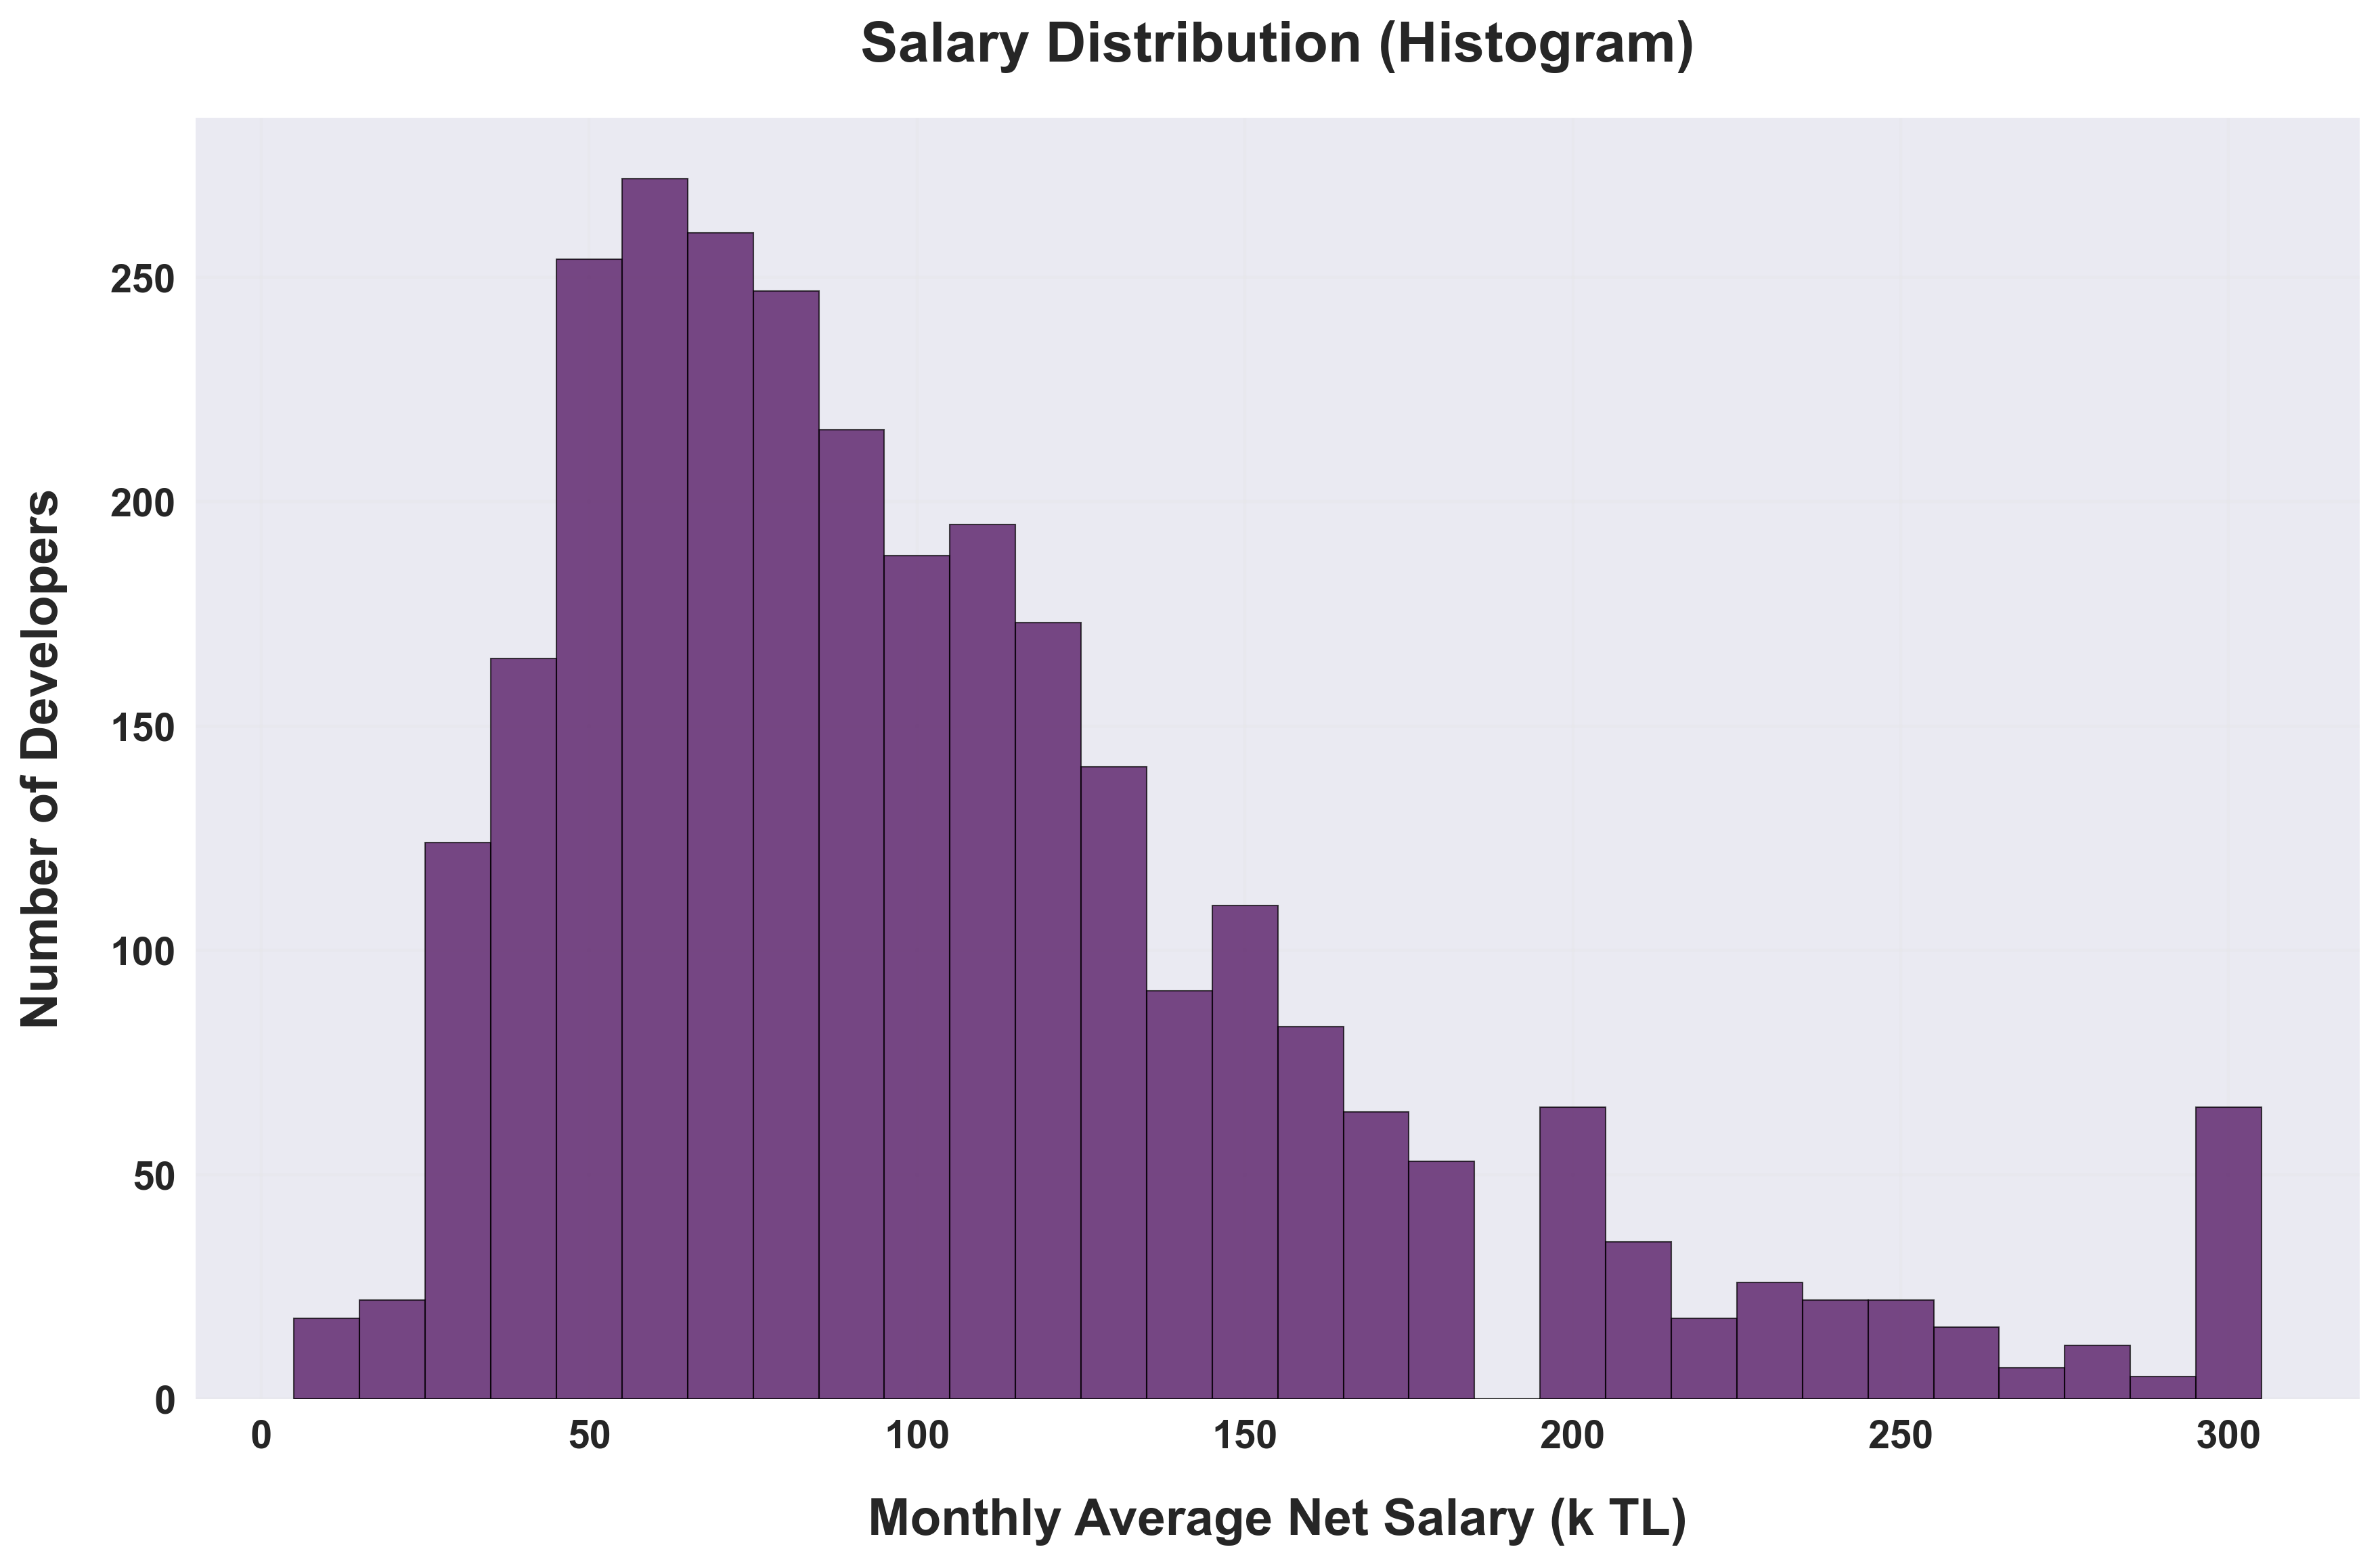
\includegraphics[width=0.85\linewidth]{figures/01_maas_dagilimi_histogram.png}
  \caption{Salary distribution (histogram with density overlay).}
  \label{fig:salary-dist}
\end{figure}

\begin{figure}[H]
  \centering
  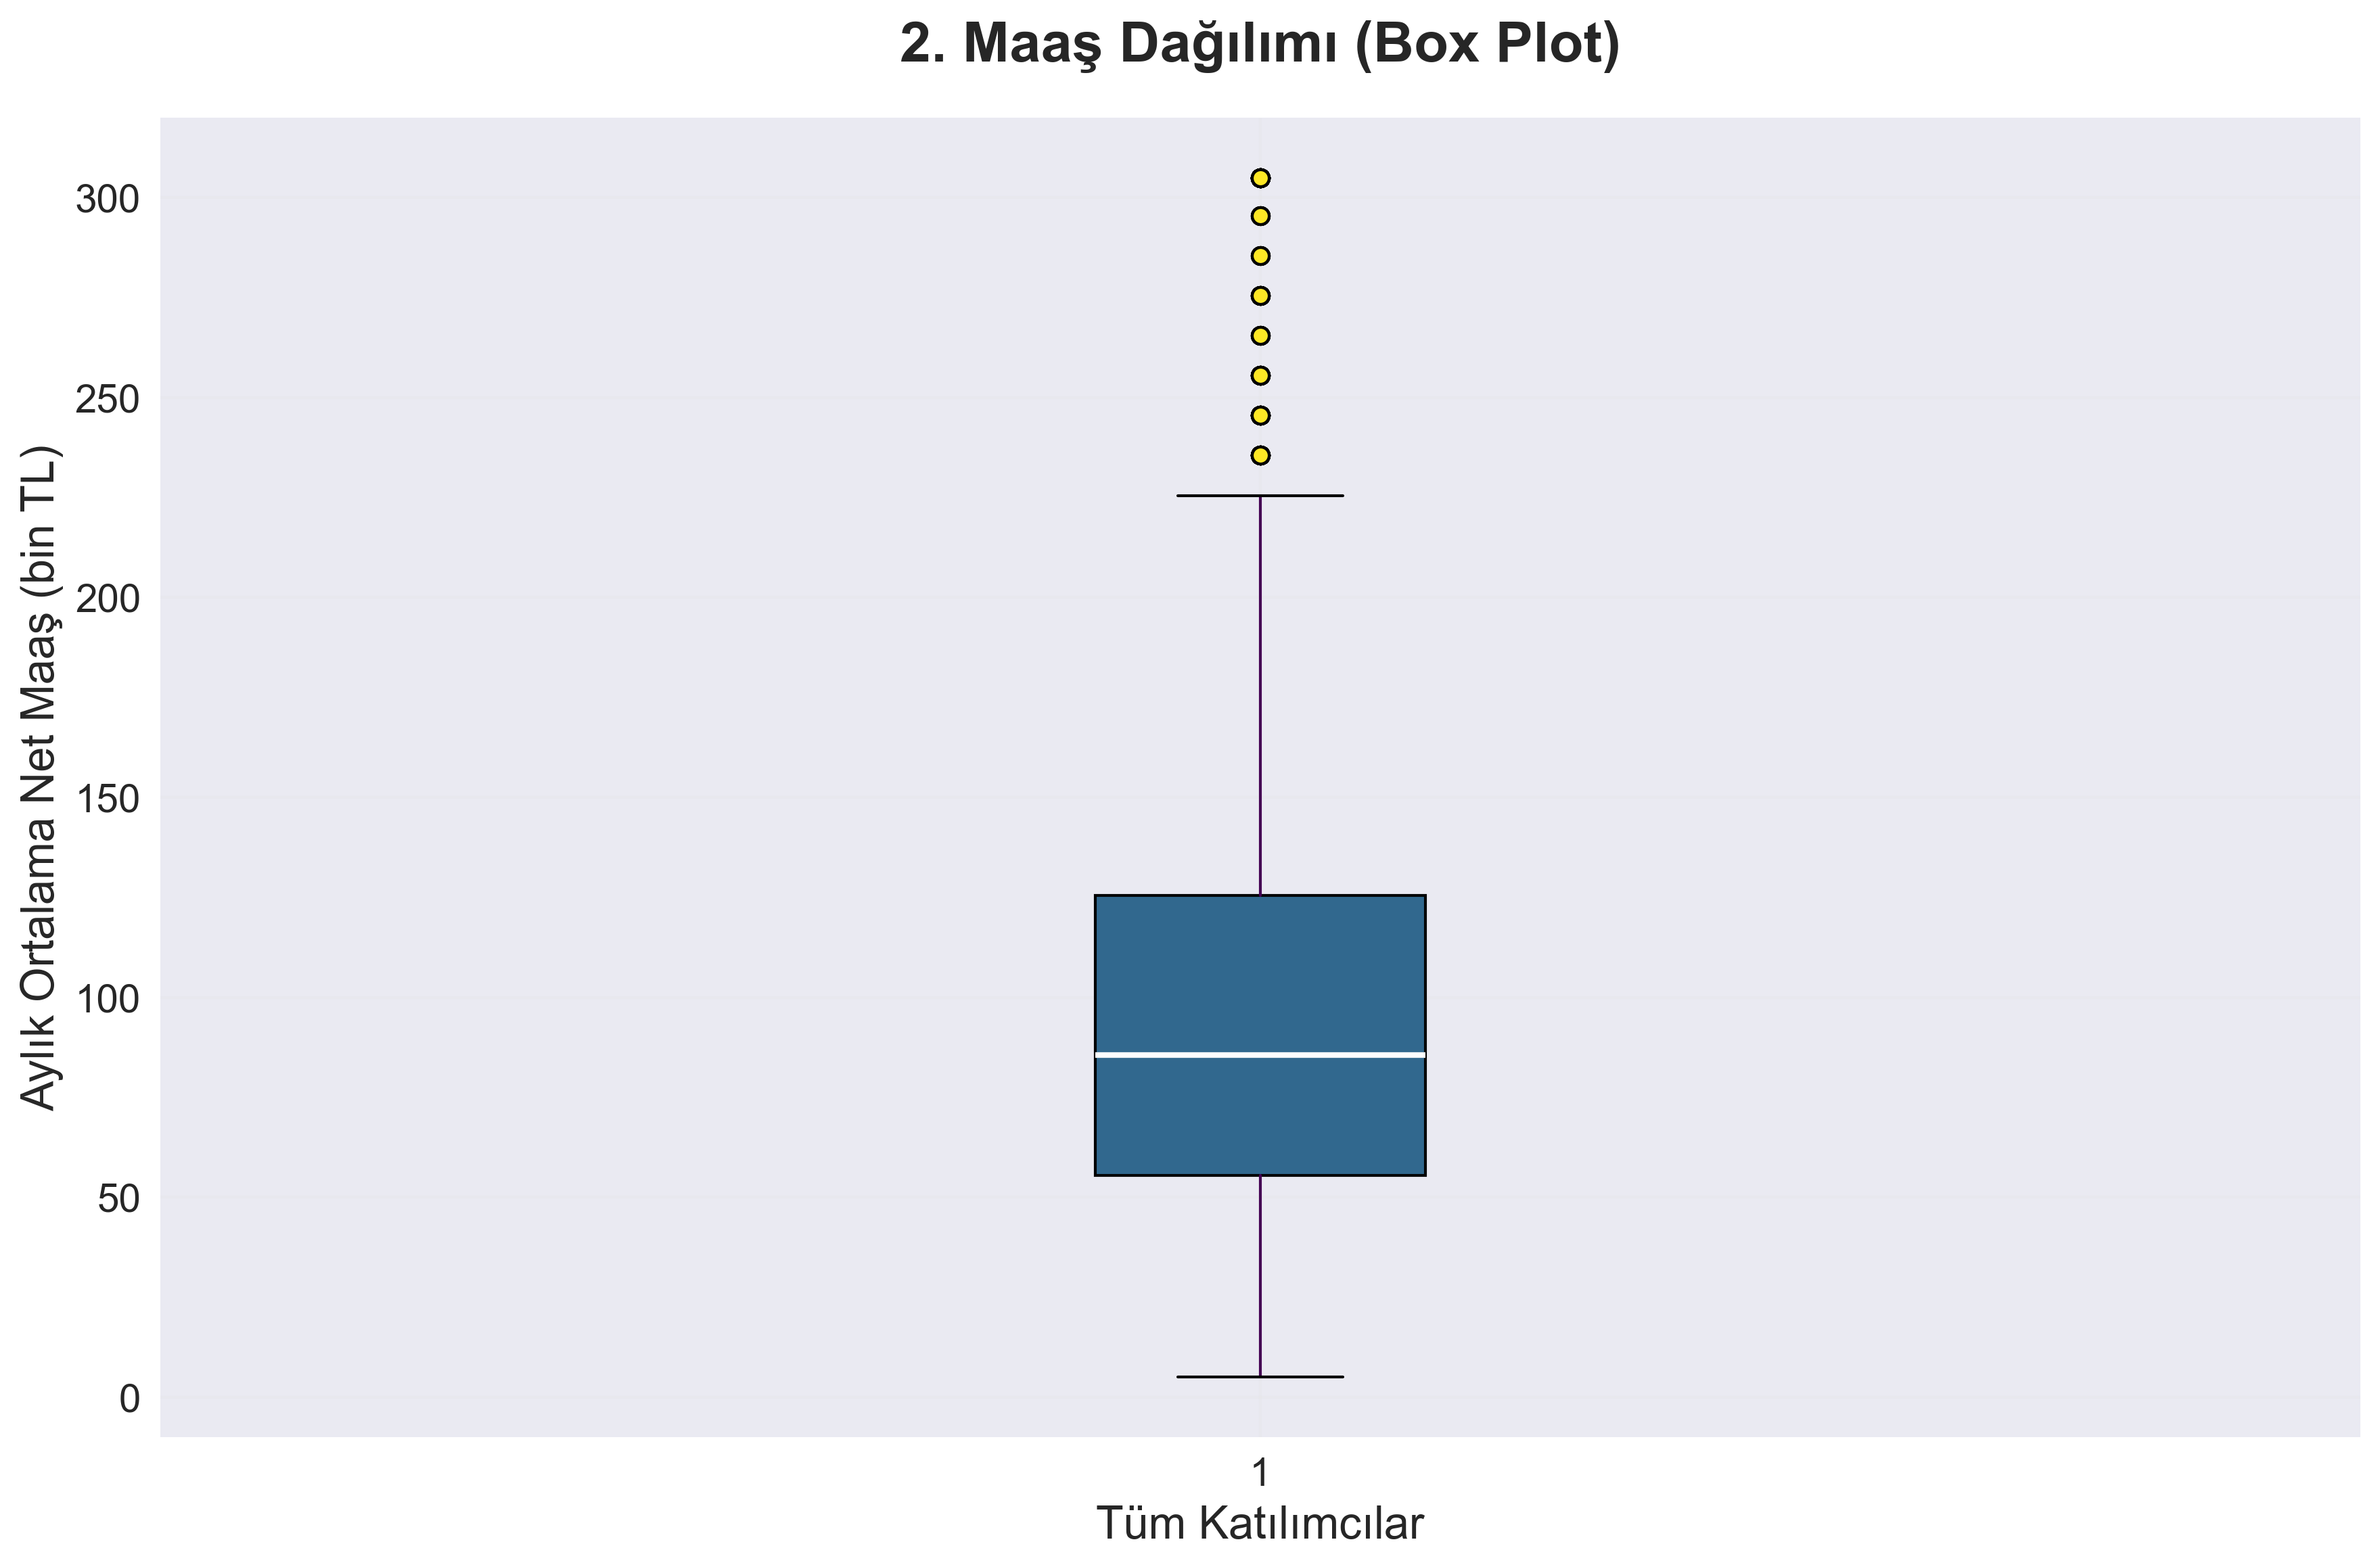
\includegraphics[width=0.85\linewidth]{figures/02_maas_dagilimi_boxplot.png}
  \caption{Salary distribution (box plot).}
  \label{fig:salary-box}
\end{figure}

\subsection{Hypothesis Testing}
Primary hypothesis tests yielded the following results:
\begin{itemize}[leftmargin=*]
  \item React vs Non-React (independent \textit{t}-test): not statistically significant ($p = 0.228$).
  \item Work arrangement (one-way ANOVA): statistically significant ($p < 0.001$), medium effect size.
  \item Company location (one-way ANOVA): statistically significant ($p < 0.001$), large effect size.
  \item Gender pay gap (independent \textit{t}-test): statistically significant ($p = 0.0004$), mean gap $\approx 16\%$.
\end{itemize}

Post-hoc comparisons (Tukey HSD) indicate differences are concentrated between remote vs office and by clusters of company locations.

\subsection{Stack ROI}
We benchmarked mean salaries by programming languages, frontend frameworks, and tools, and summarized relative effect sizes as a qualitative ROI ranking. Stacks combining modern frontend and robust backend competencies tend to outperform single-technology profiles. Figure~\ref{fig:stack-roi} shows the ranked comparison.

\begin{figure}[H]
  \centering
  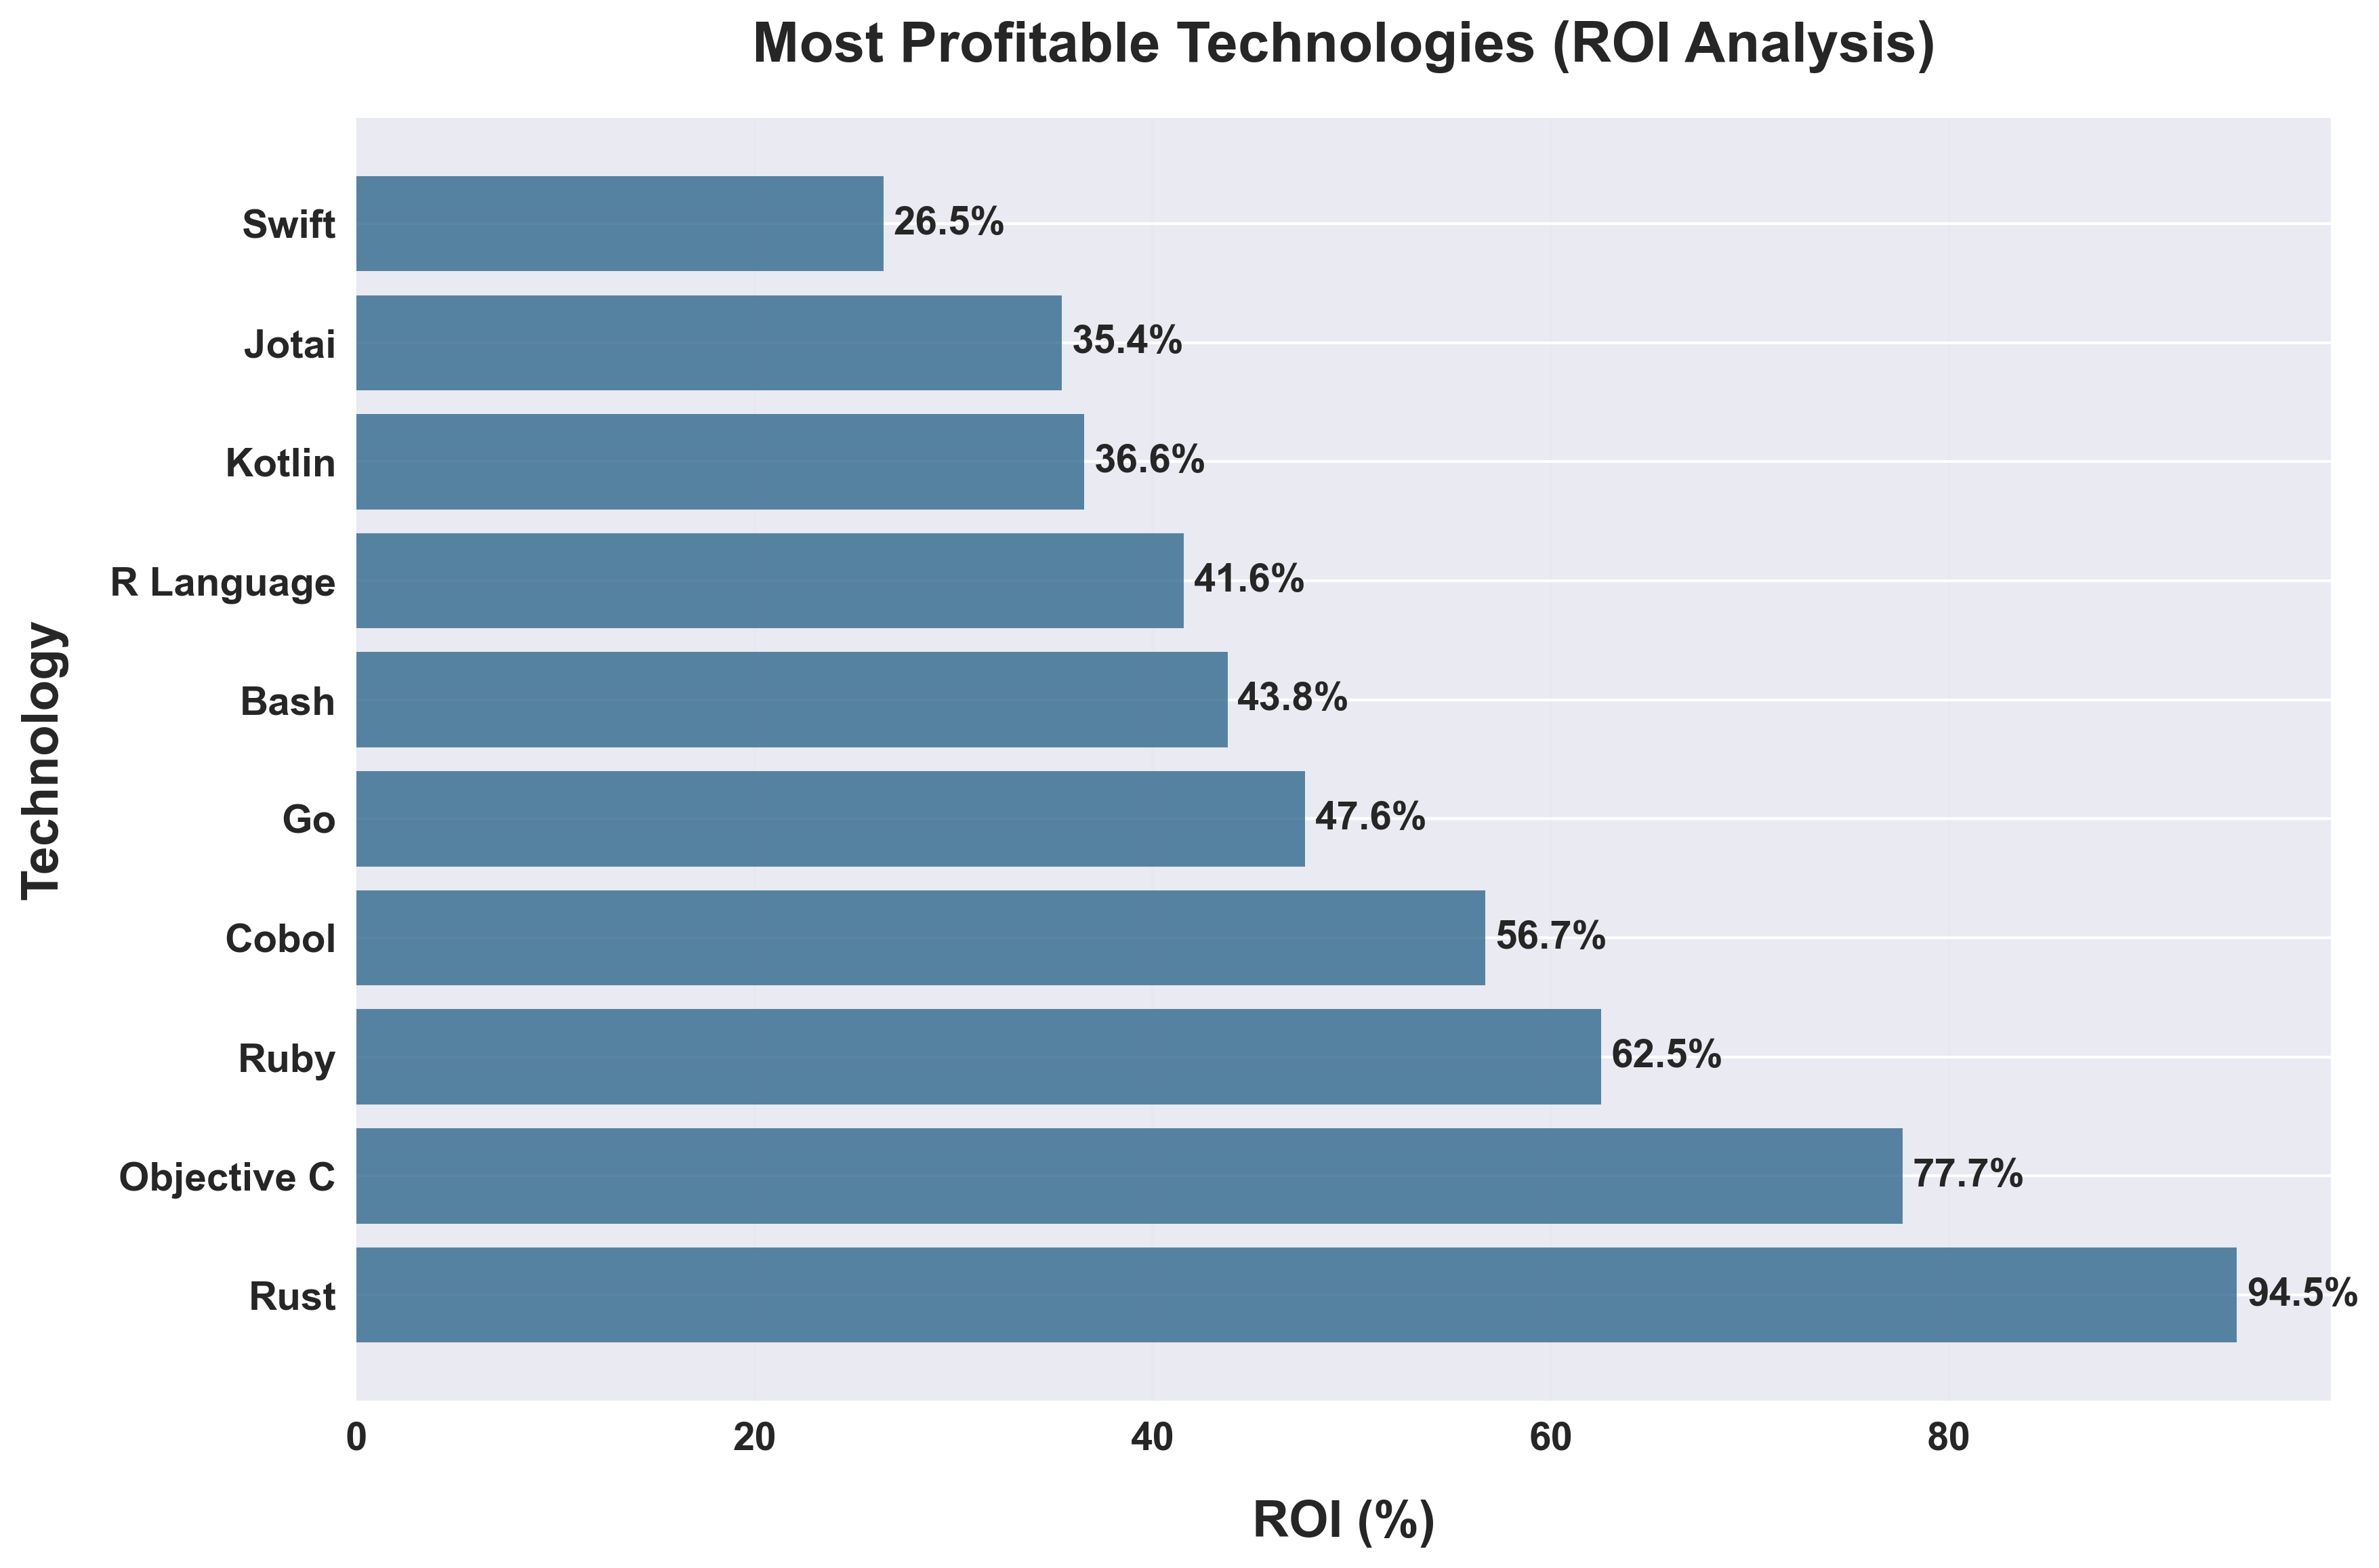
\includegraphics[width=0.85\linewidth]{figures/12_en_karli_teknolojiler.png}
  \caption{Relative ROI by technology stack.}
  \label{fig:stack-roi}
\end{figure}

\subsection{Additional Visualizations}
We include a non-exhaustive set of publication-quality charts to illustrate key relationships:

\begin{figure}[H]
  \centering
  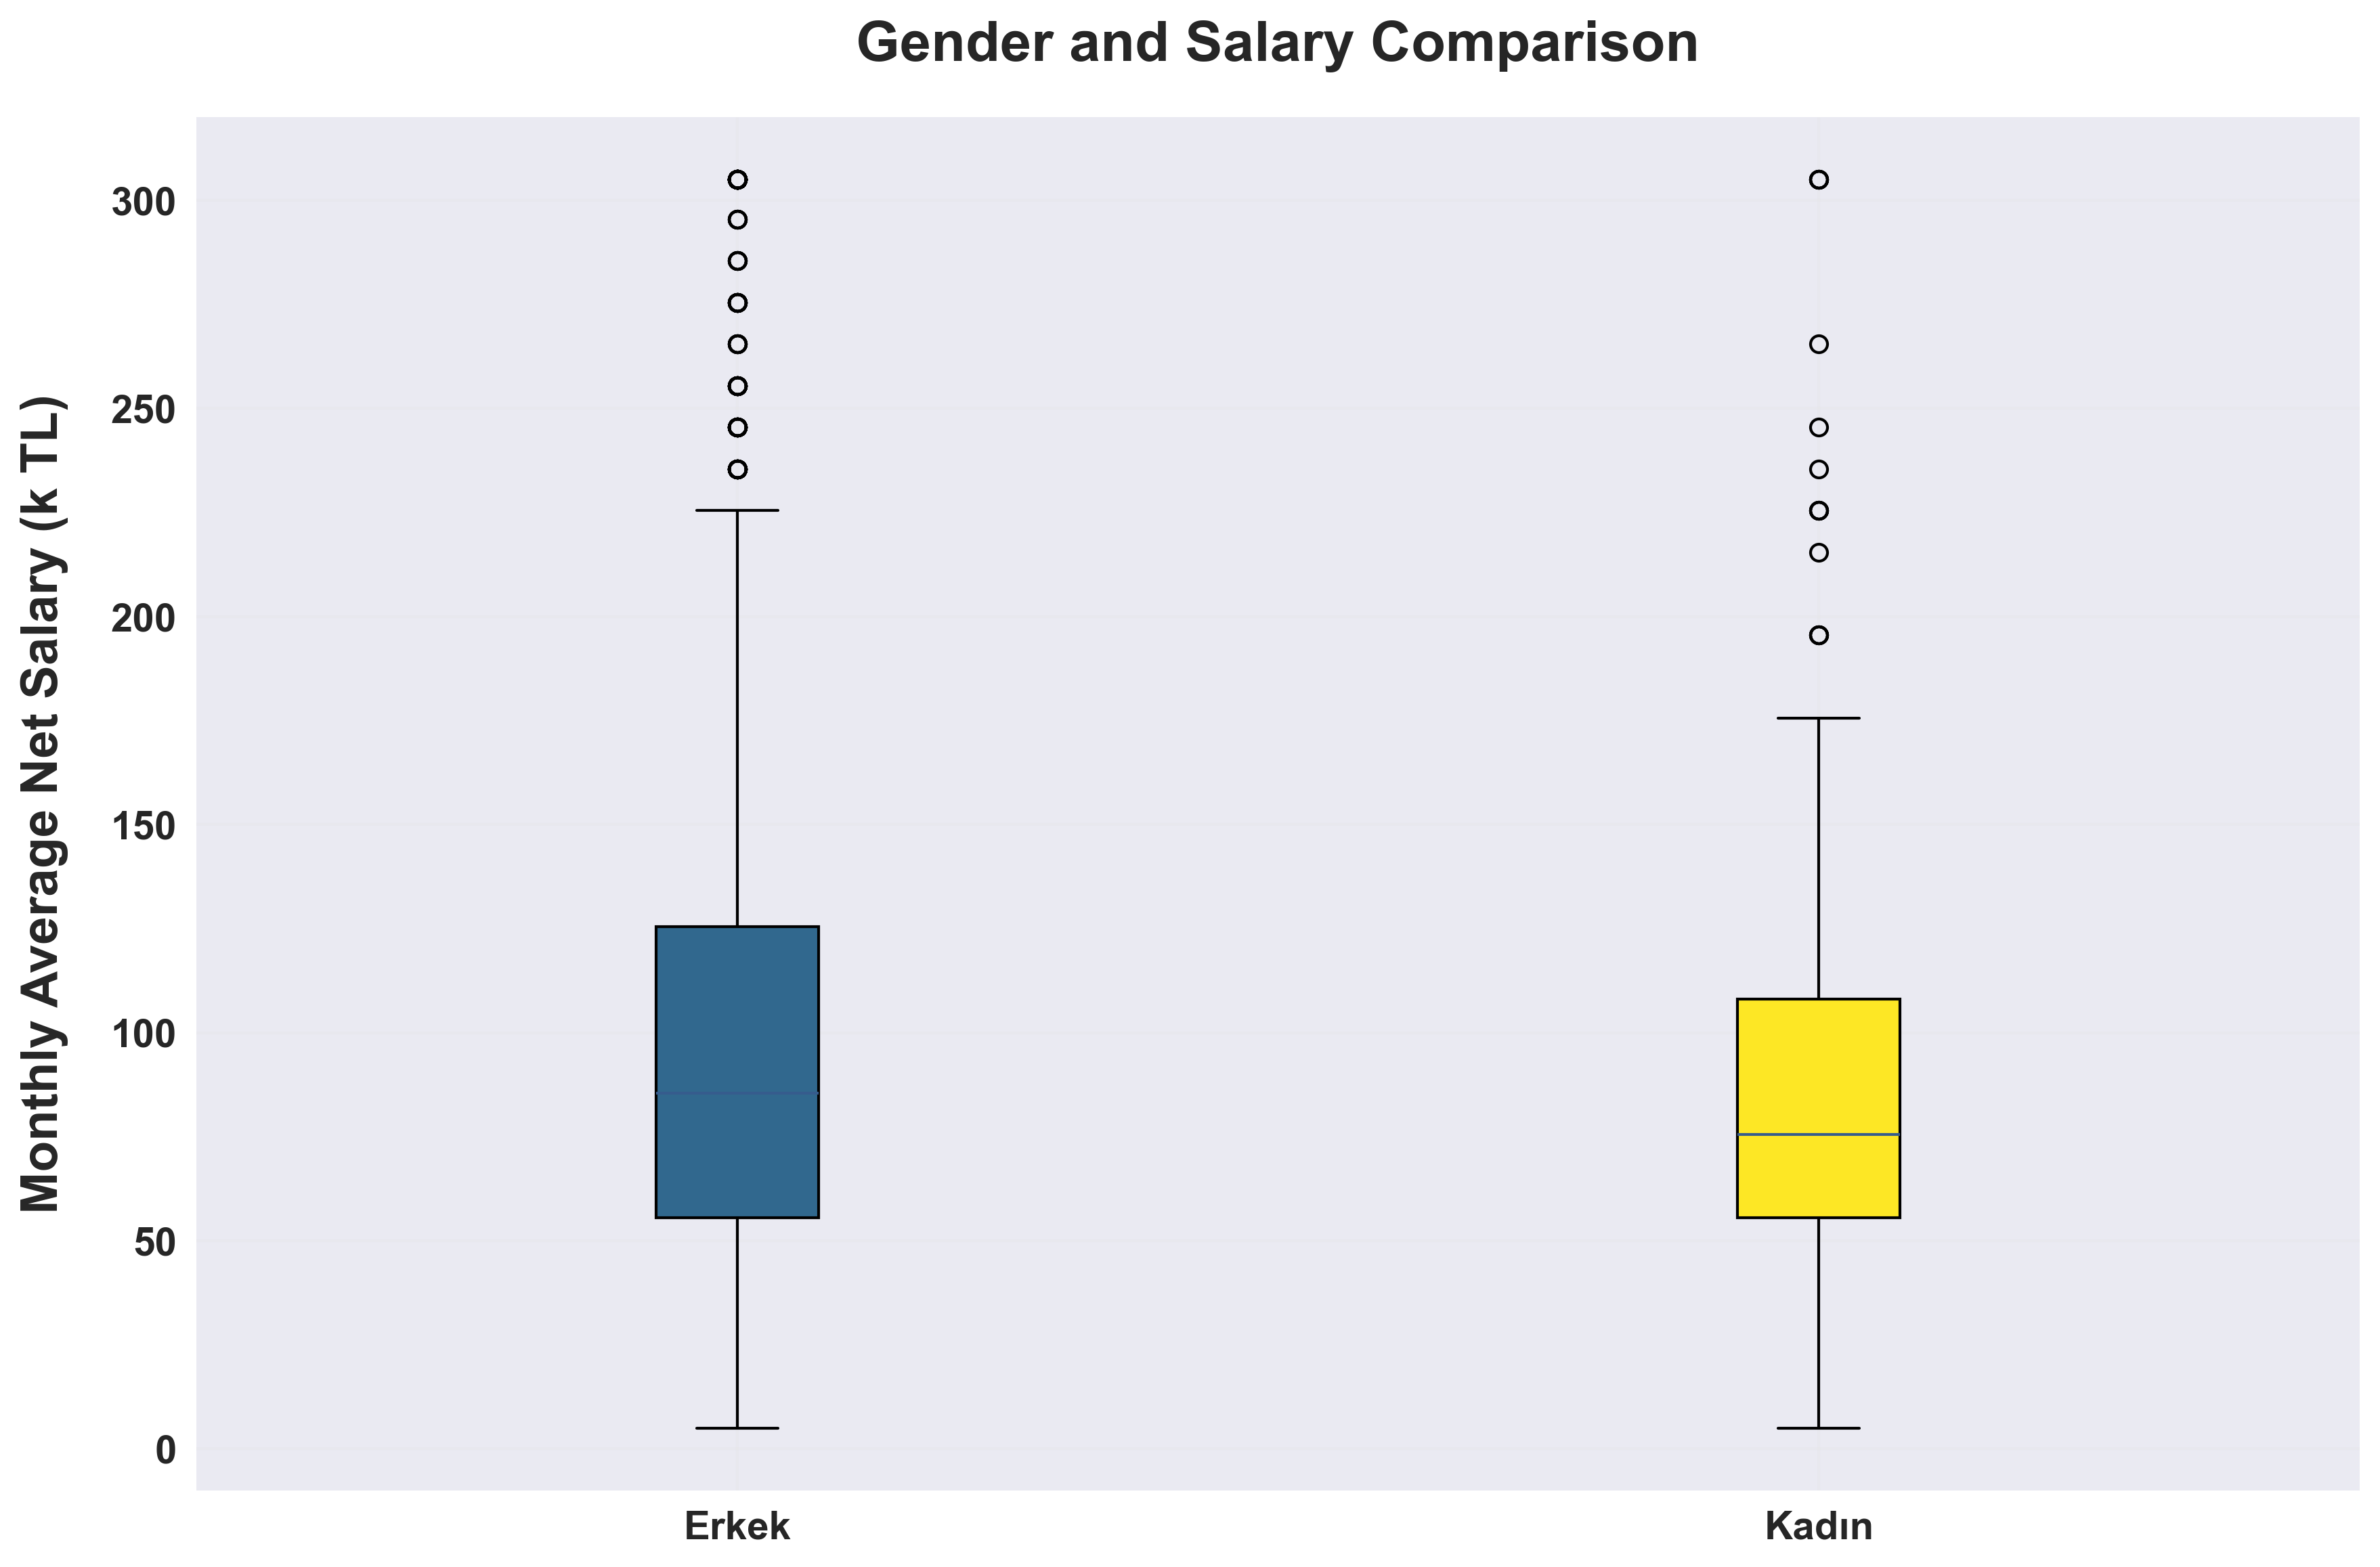
\includegraphics[width=0.85\linewidth]{figures/06_cinsiyet_maas_karsilastirma.png}
  \caption{Gender-based salary comparison.}
  \label{fig:gender-gap}
\end{figure}

\begin{figure}[H]
  \centering
  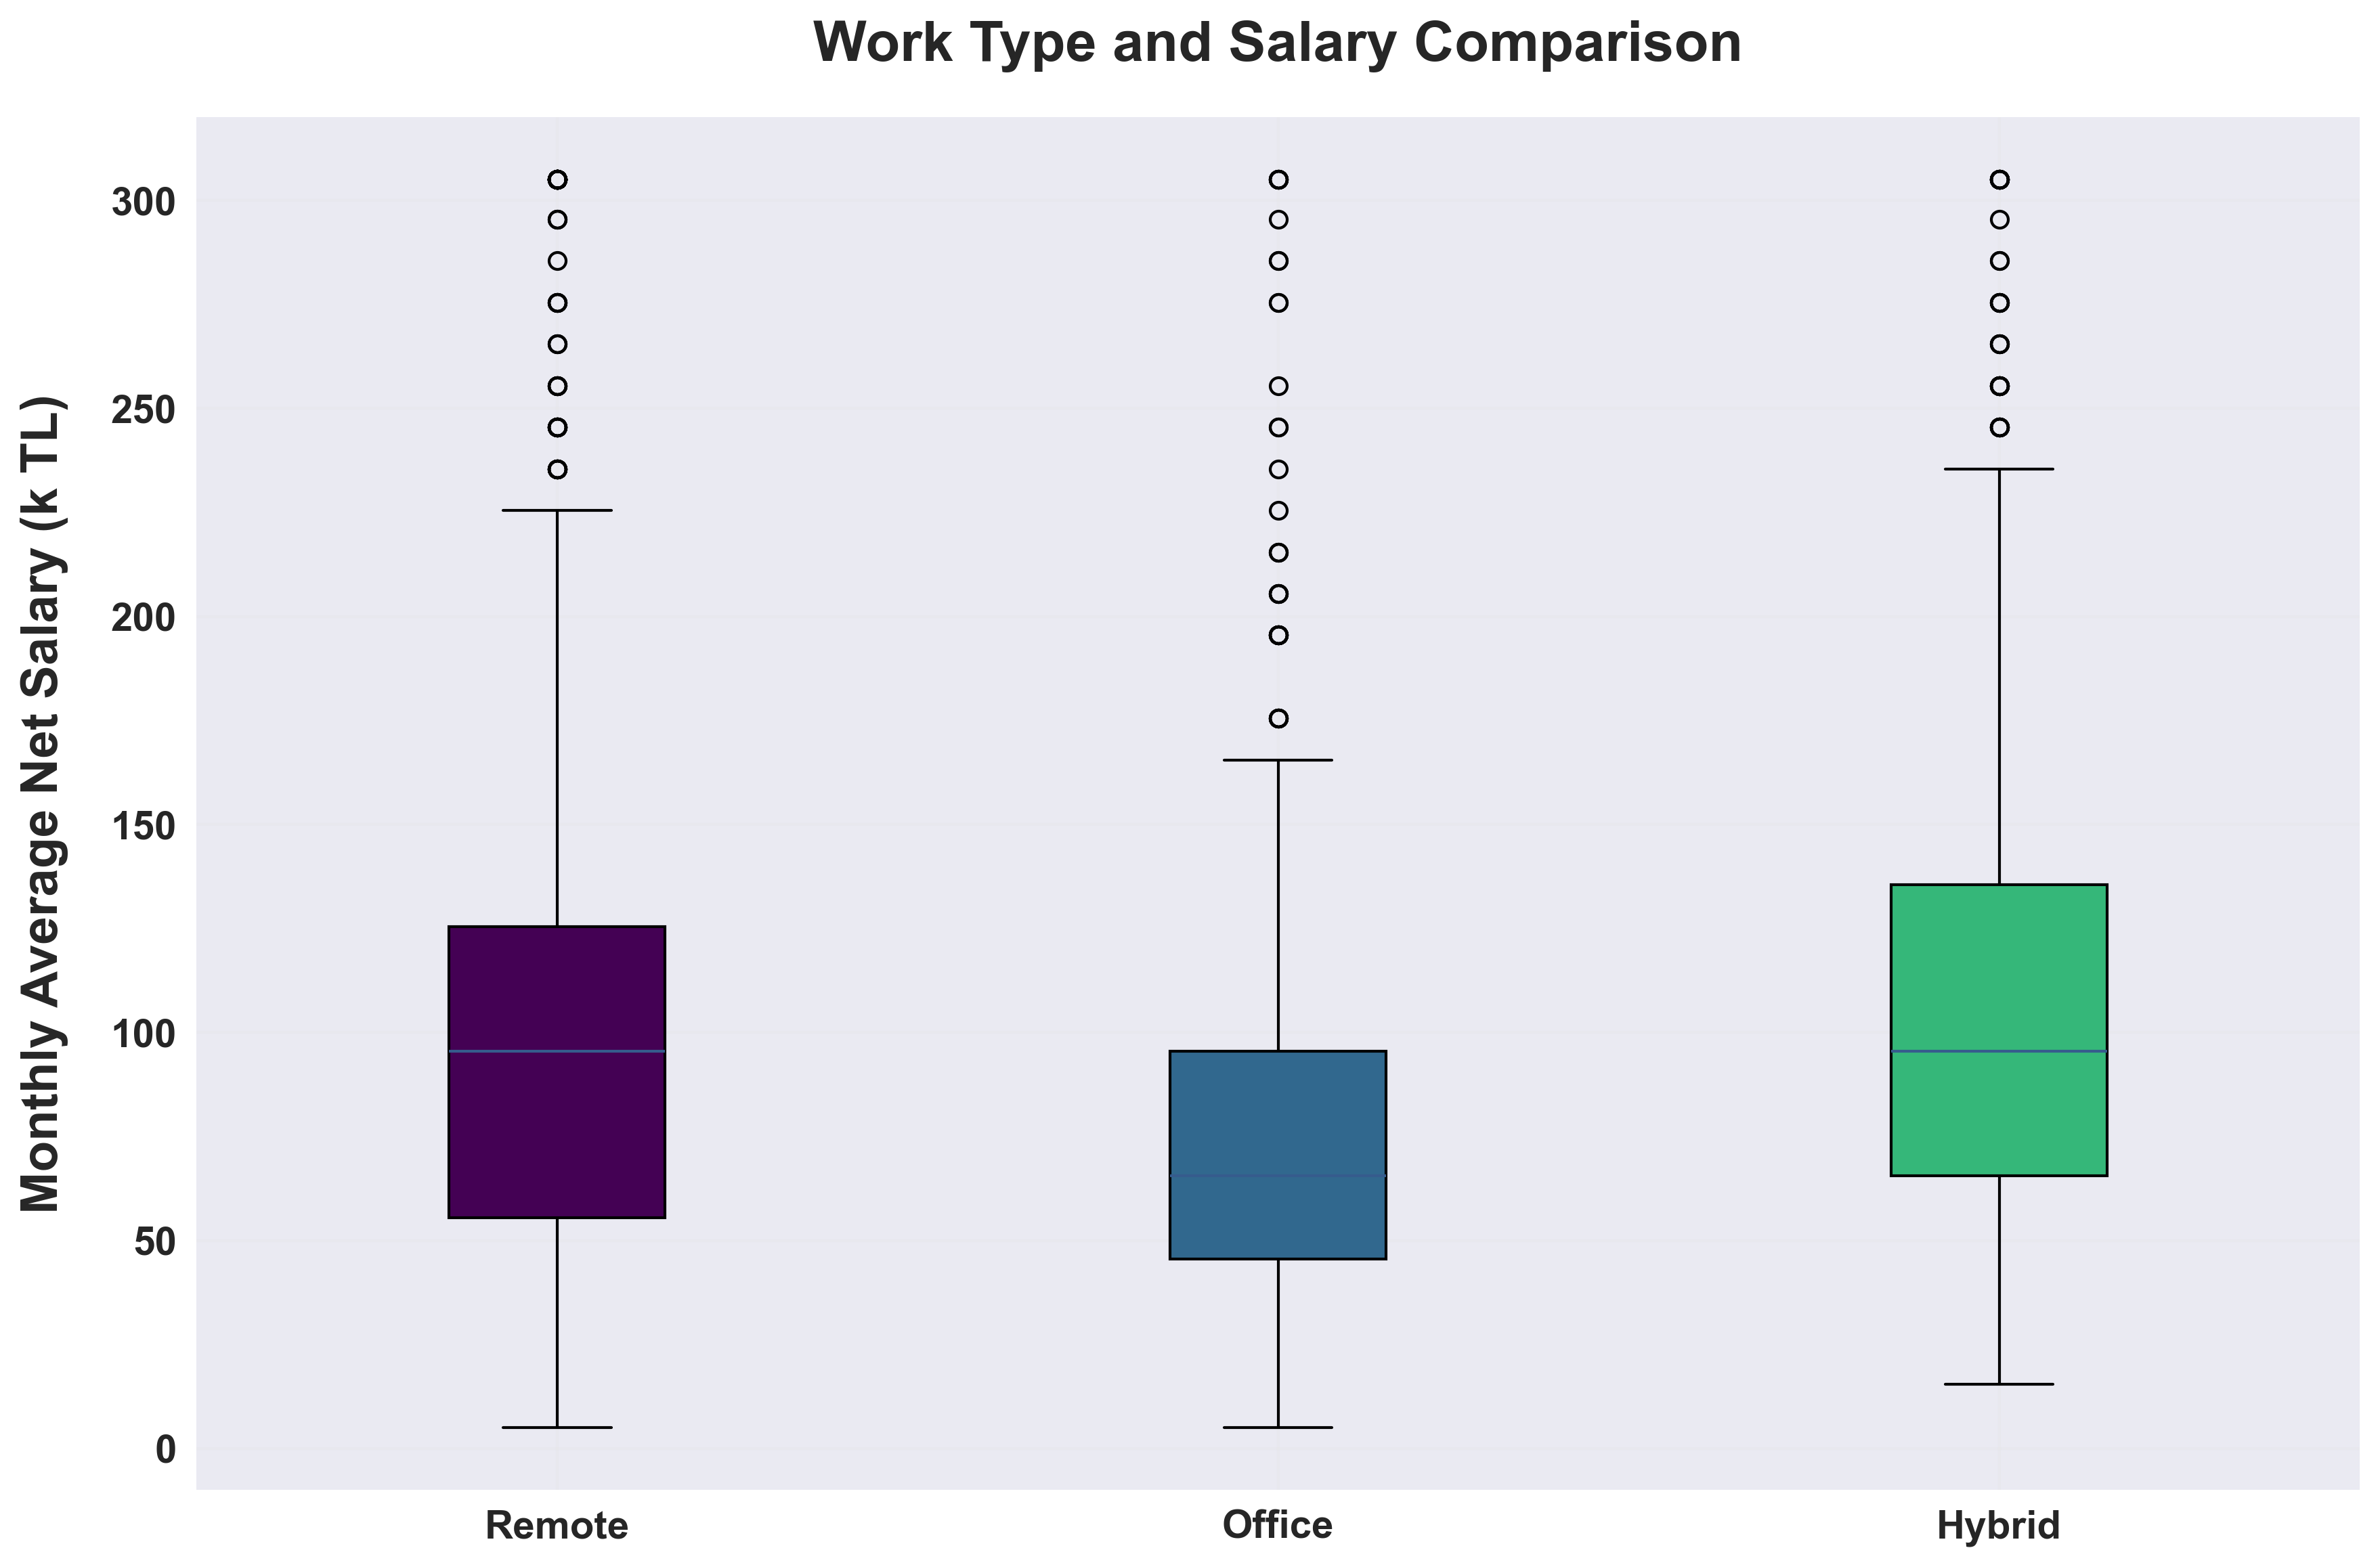
\includegraphics[width=0.85\linewidth]{figures/07_calisma_sekli_maas_karsilastirma.png}
  \caption{Salary by work arrangement (remote, office, hybrid).}
  \label{fig:work-type}
\end{figure}

\begin{figure}[H]
  \centering
  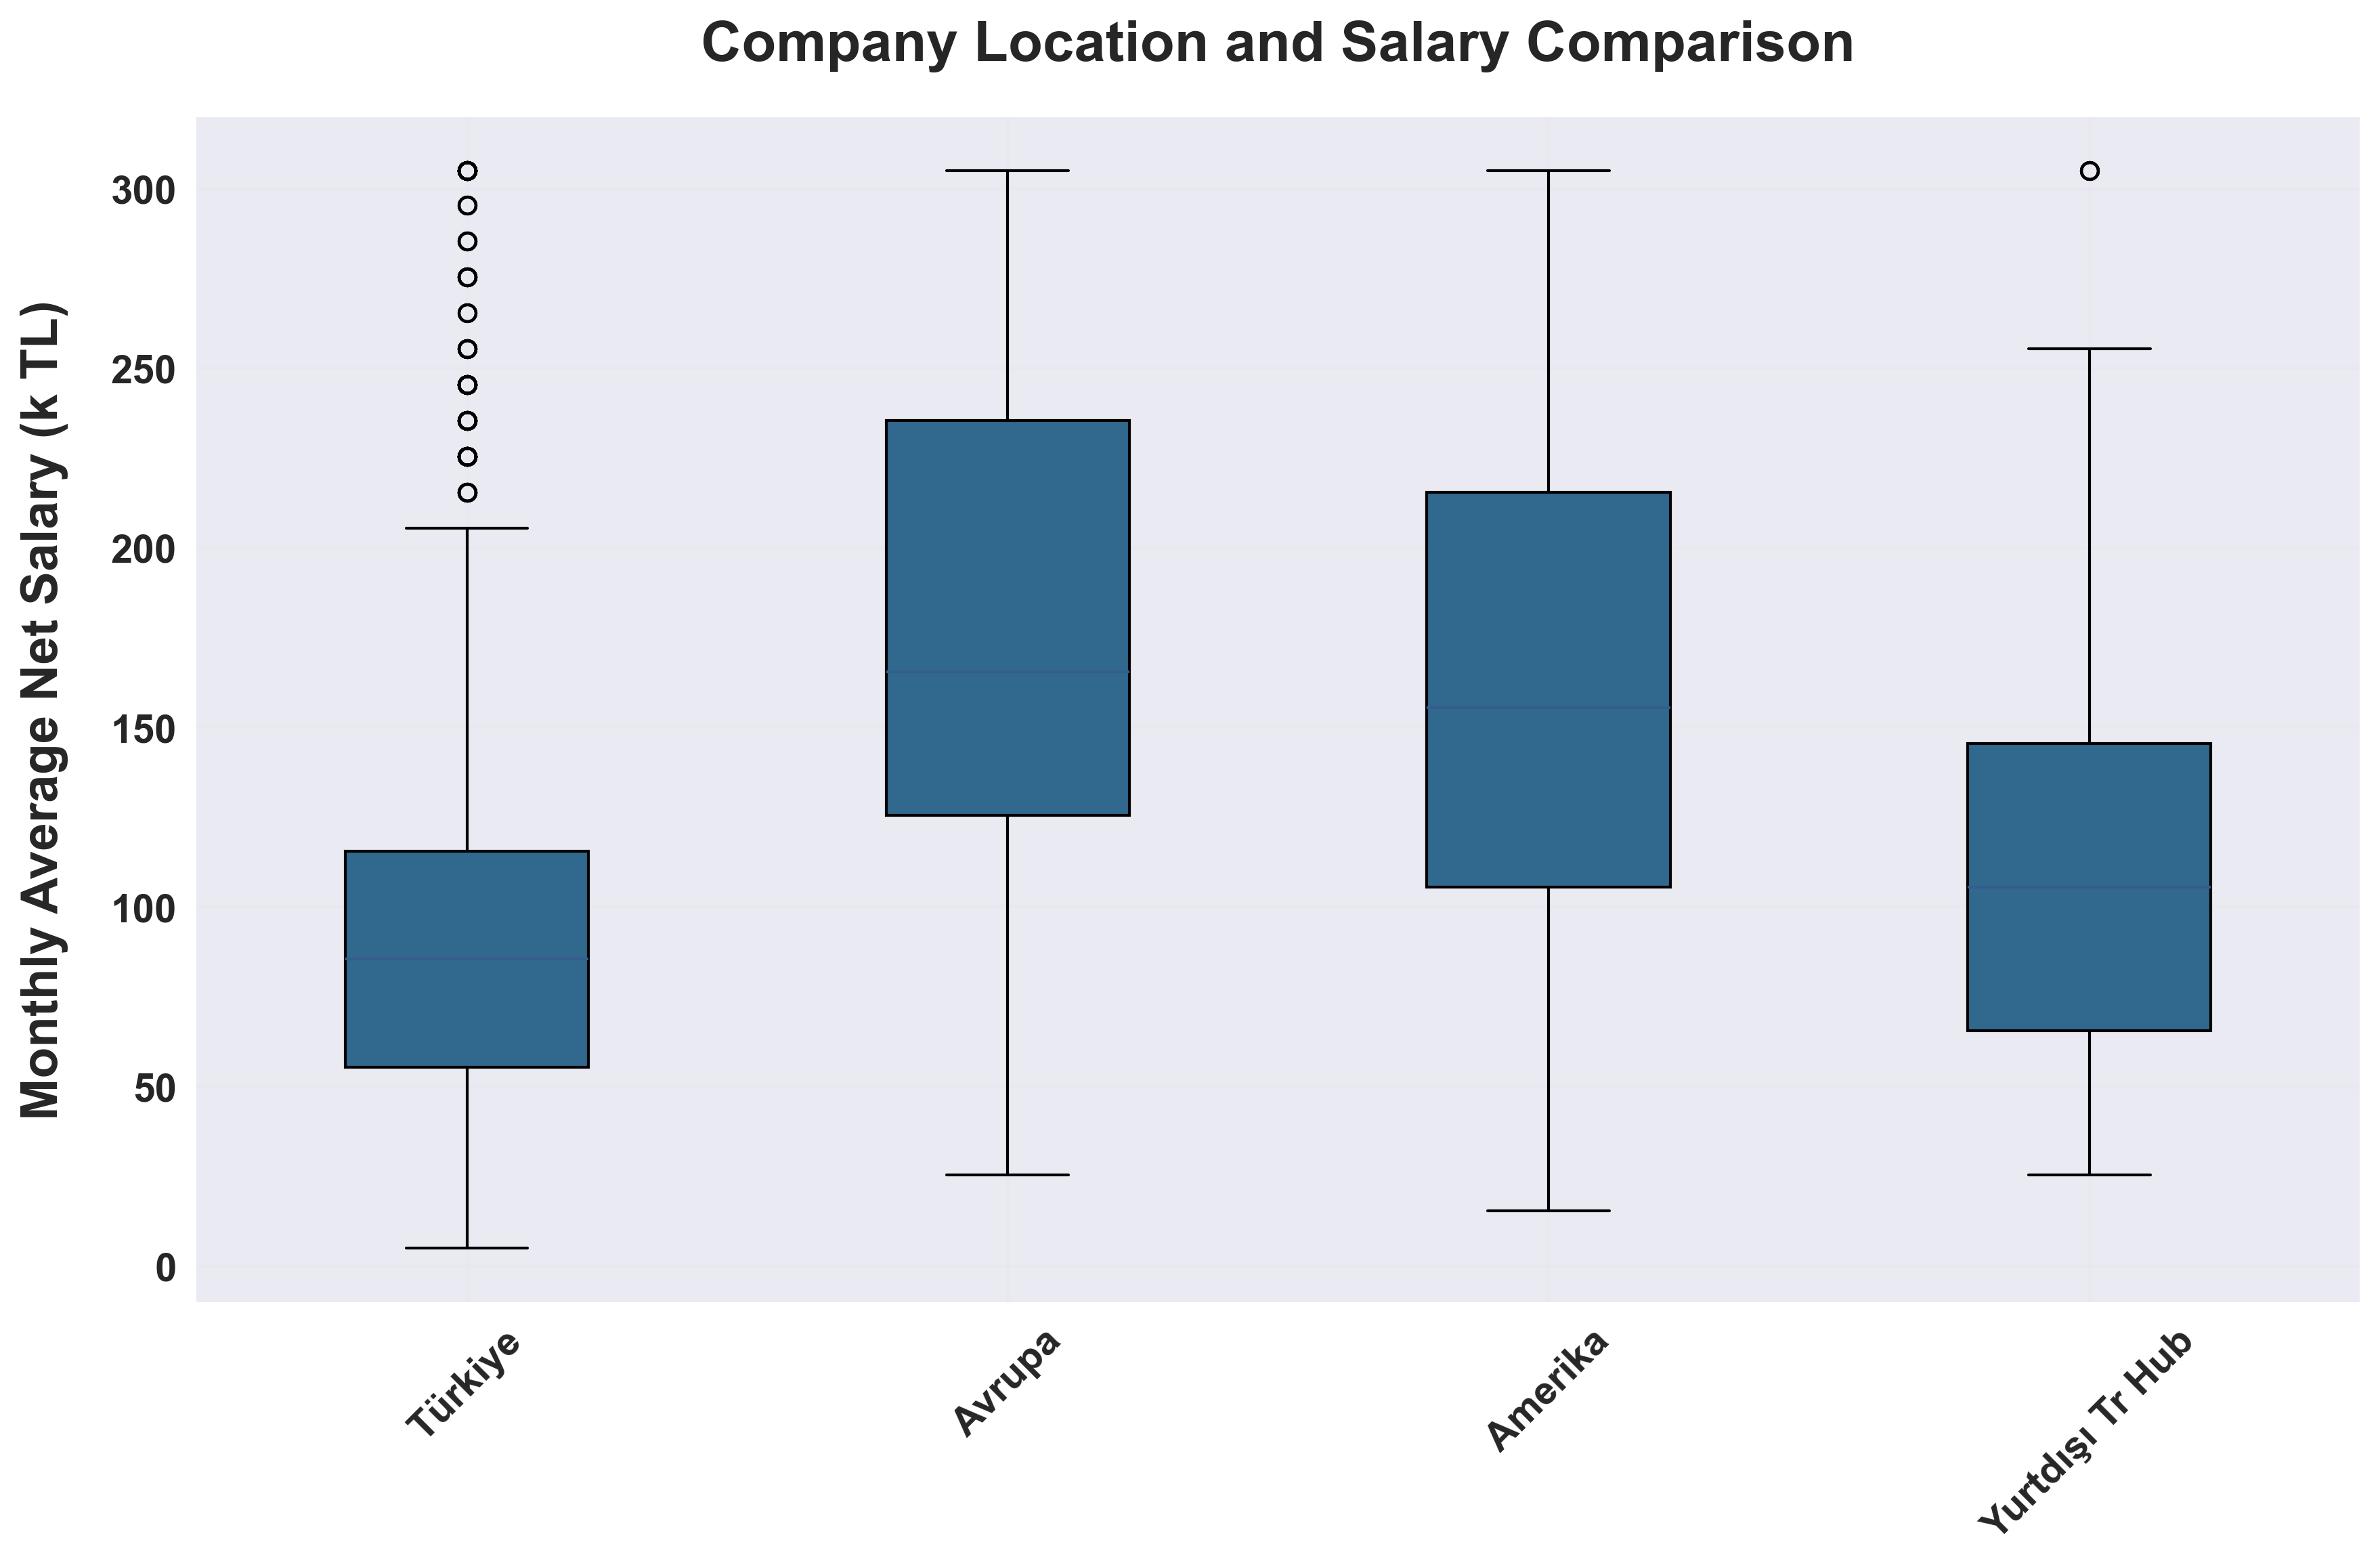
\includegraphics[width=0.85\linewidth]{figures/08_sirket_lokasyonu_maas_karsilastirma.png}
  \caption{Salary by company location.}
  \label{fig:location}
\end{figure}

\begin{figure}[H]
  \centering
  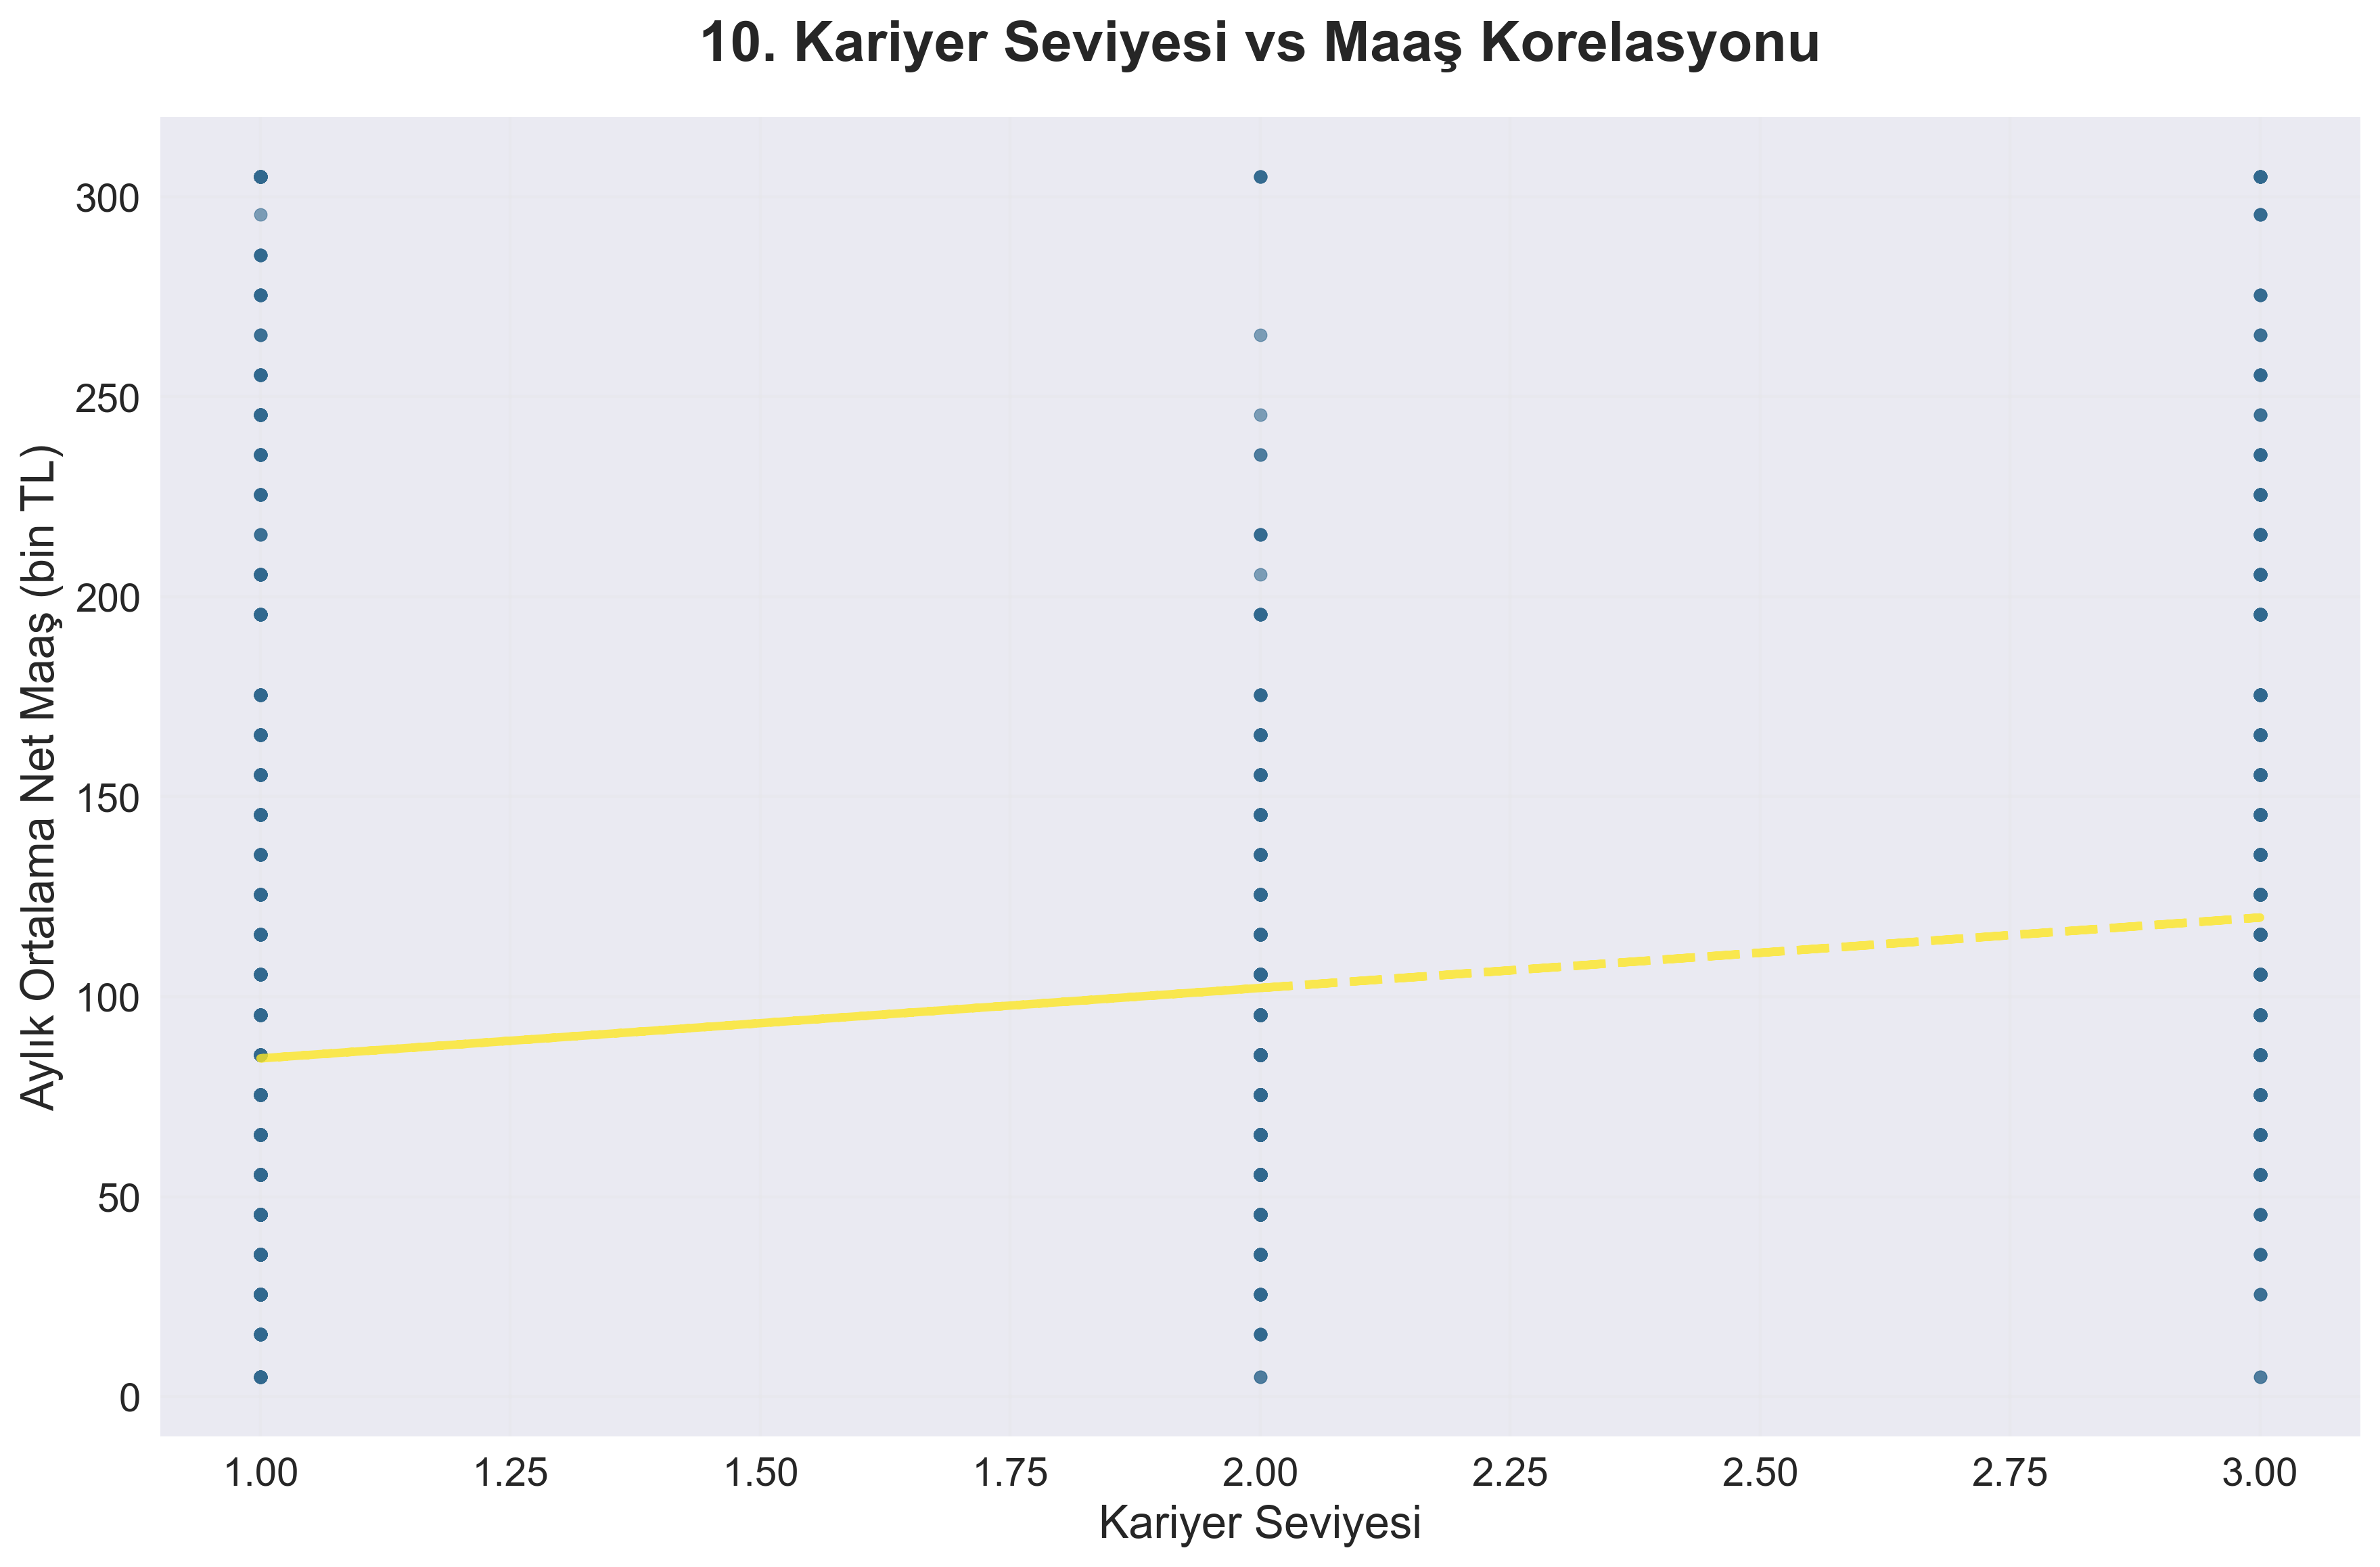
\includegraphics[width=0.85\linewidth]{figures/10_deneyim_maas_scatter.png}
  \caption{Experience vs salary (scatter).}
  \label{fig:experience}
\end{figure}

% New engaging figures
\begin{figure}[H]
  \centering
  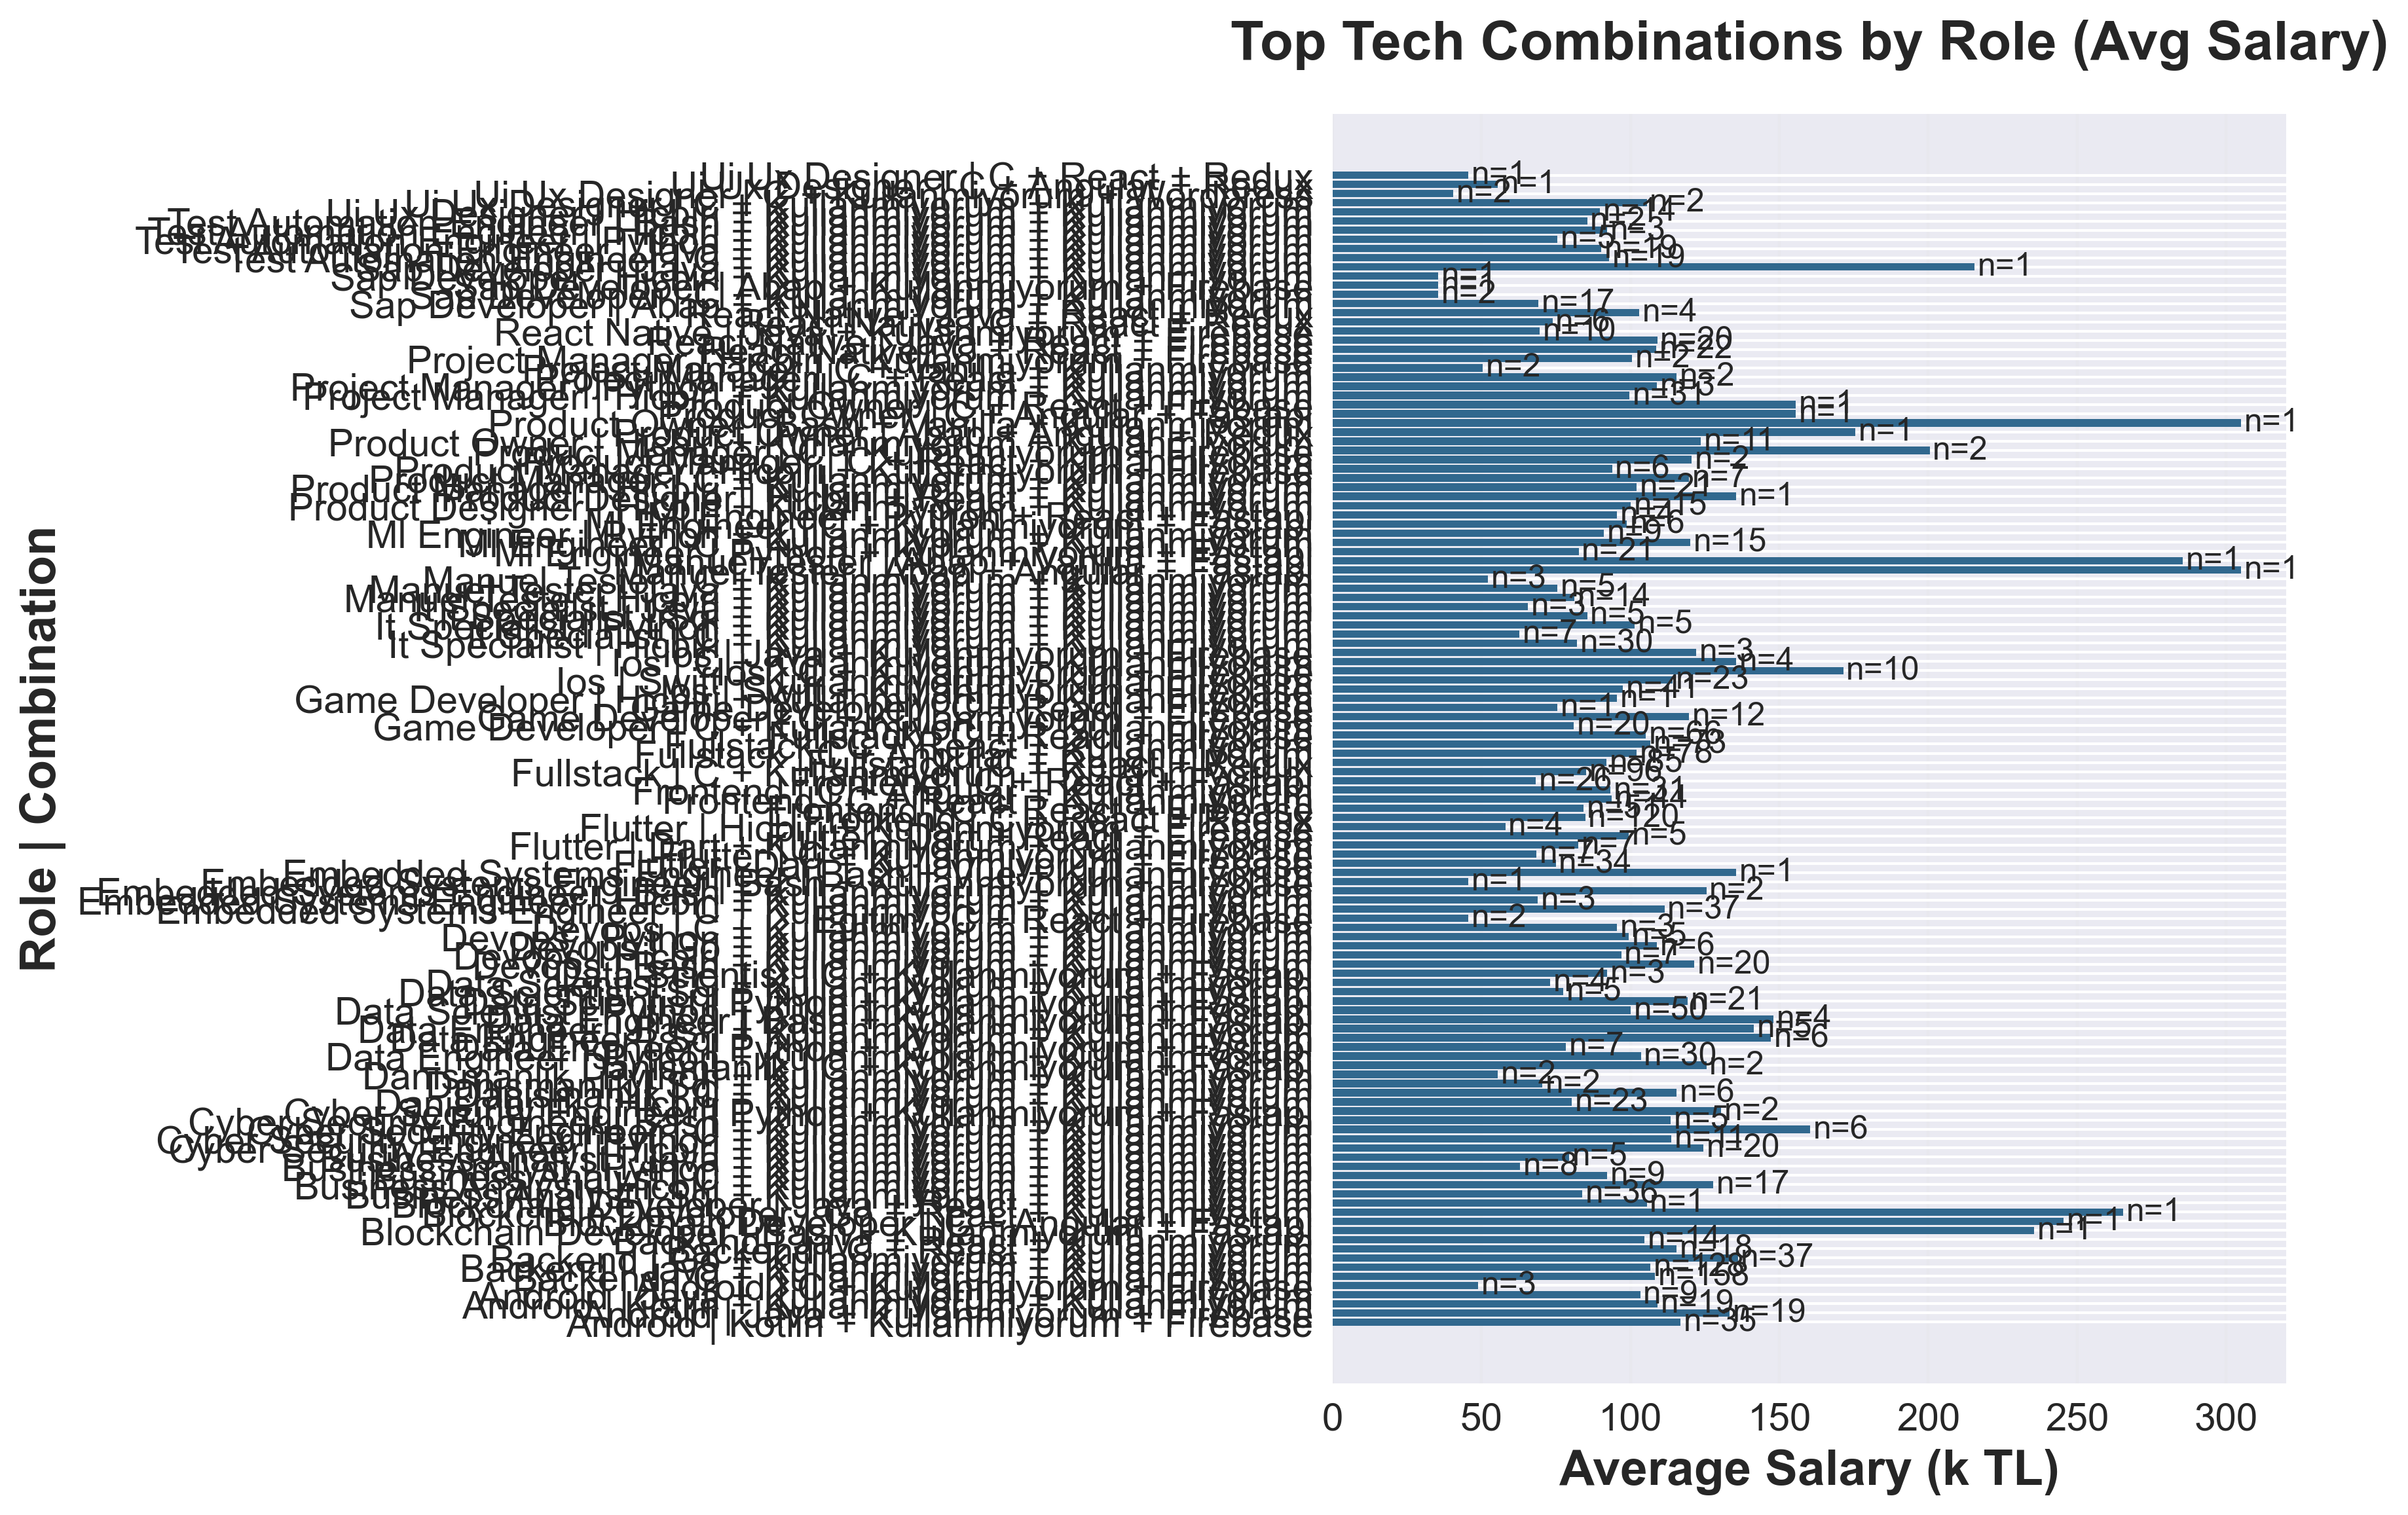
\includegraphics[width=0.85\linewidth]{figures/21_tech_combo_top.png}
  \caption{Top tech combinations by role with average salaries.}
  \label{fig:tech-combos}
\end{figure}

\begin{figure}[H]
  \centering
  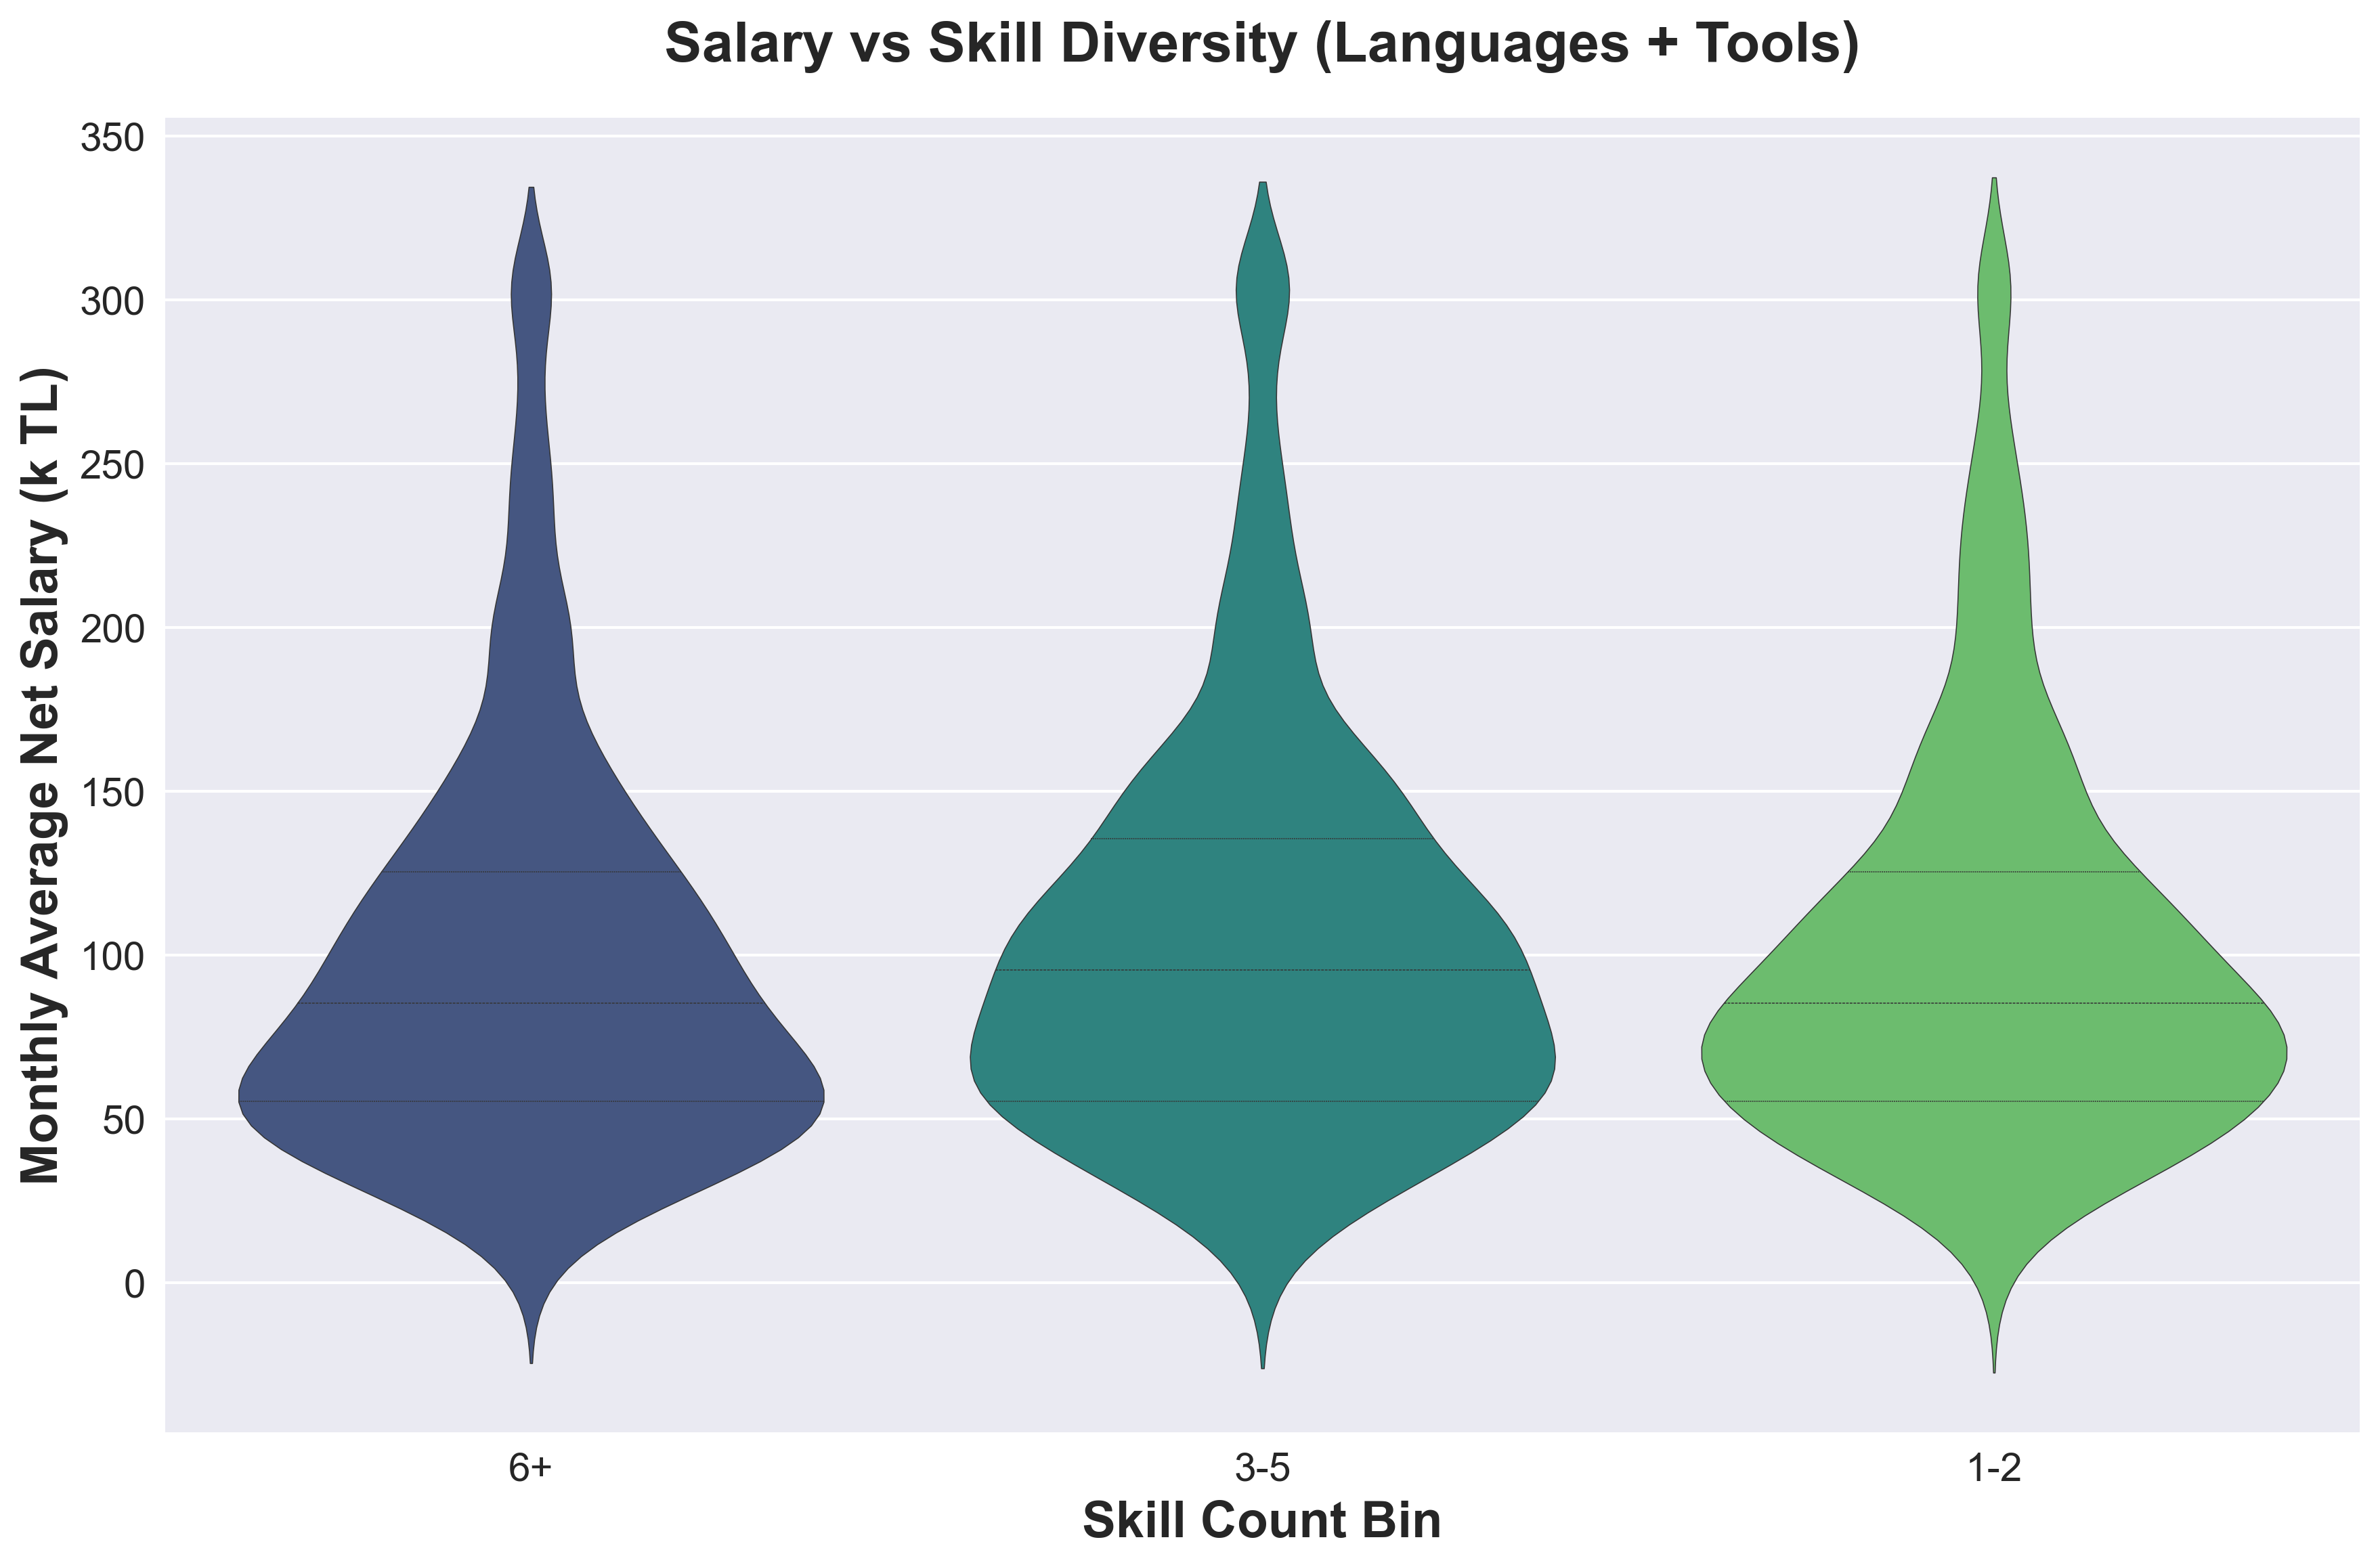
\includegraphics[width=0.85\linewidth]{figures/22_skill_diversity_salary.png}
  \caption{Salary distribution by skill diversity (languages + tools).}
  \label{fig:skill-diversity}
\end{figure}

\begin{figure}[H]
  \centering
  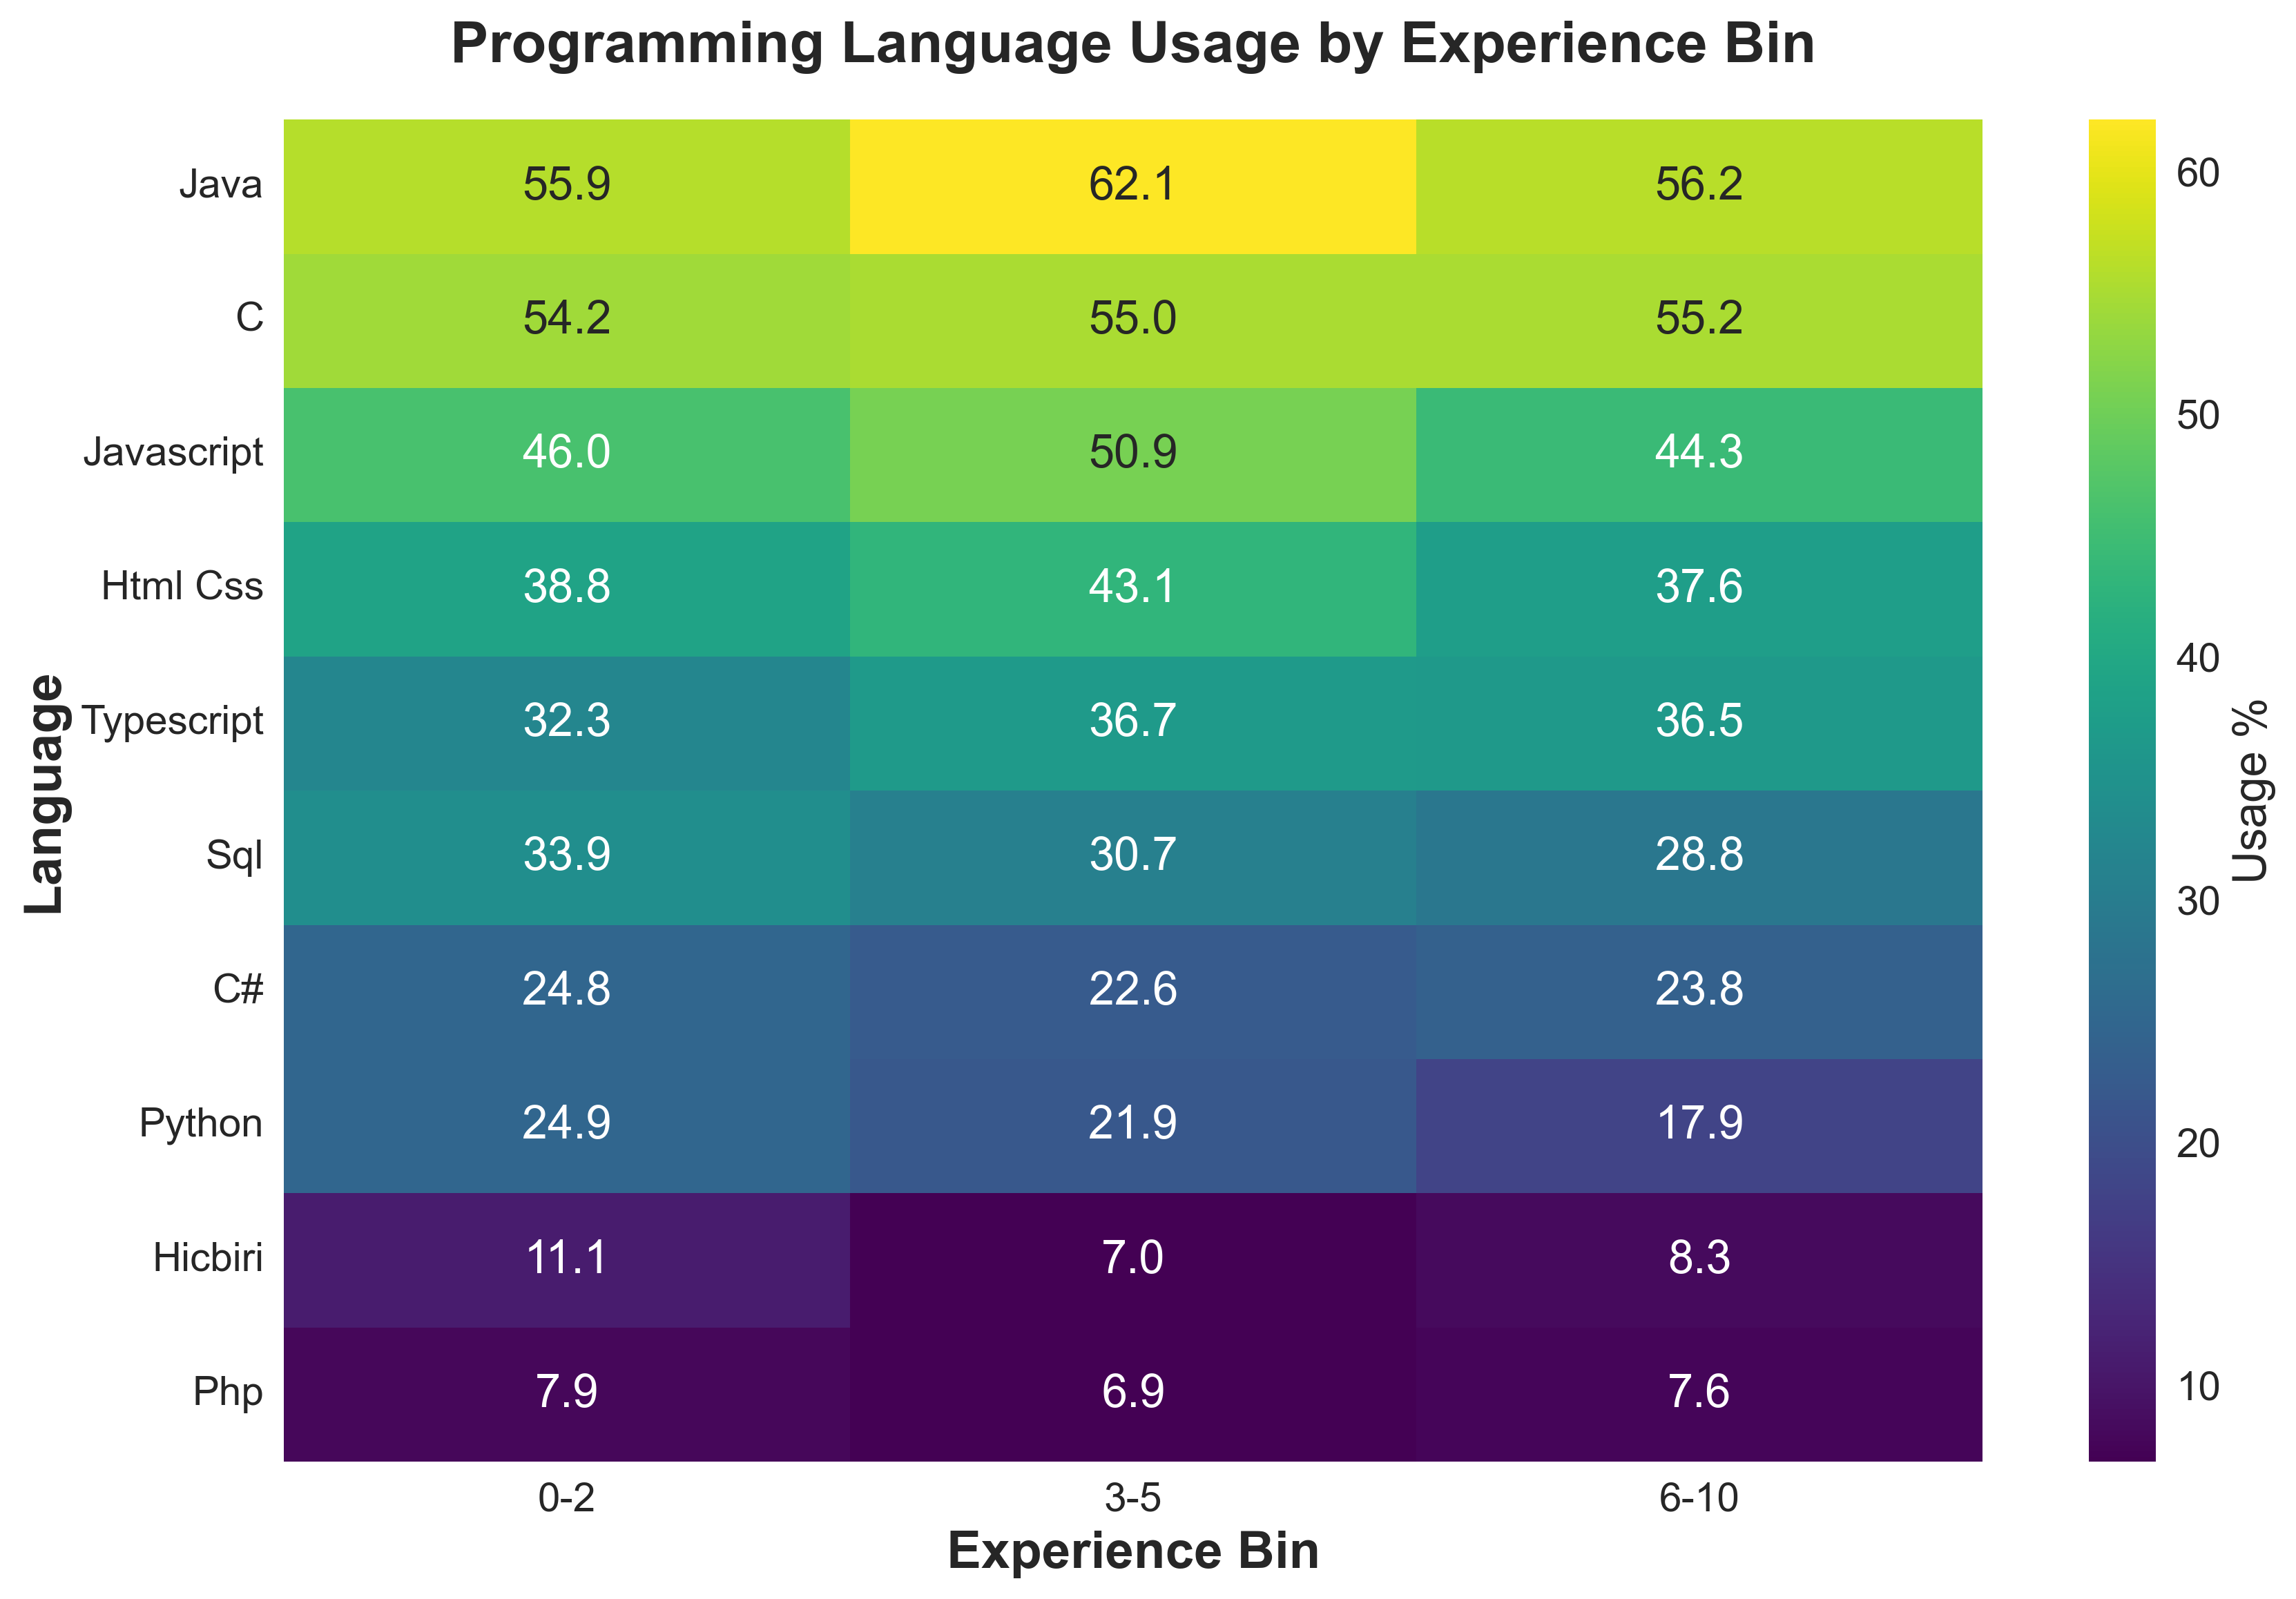
\includegraphics[width=0.85\linewidth]{figures/23_experience_lang_usage_heatmap.png}
  \caption{Programming language usage by experience bin.}
  \label{fig:exp-usage}
\end{figure}

\begin{figure}[H]
  \centering
  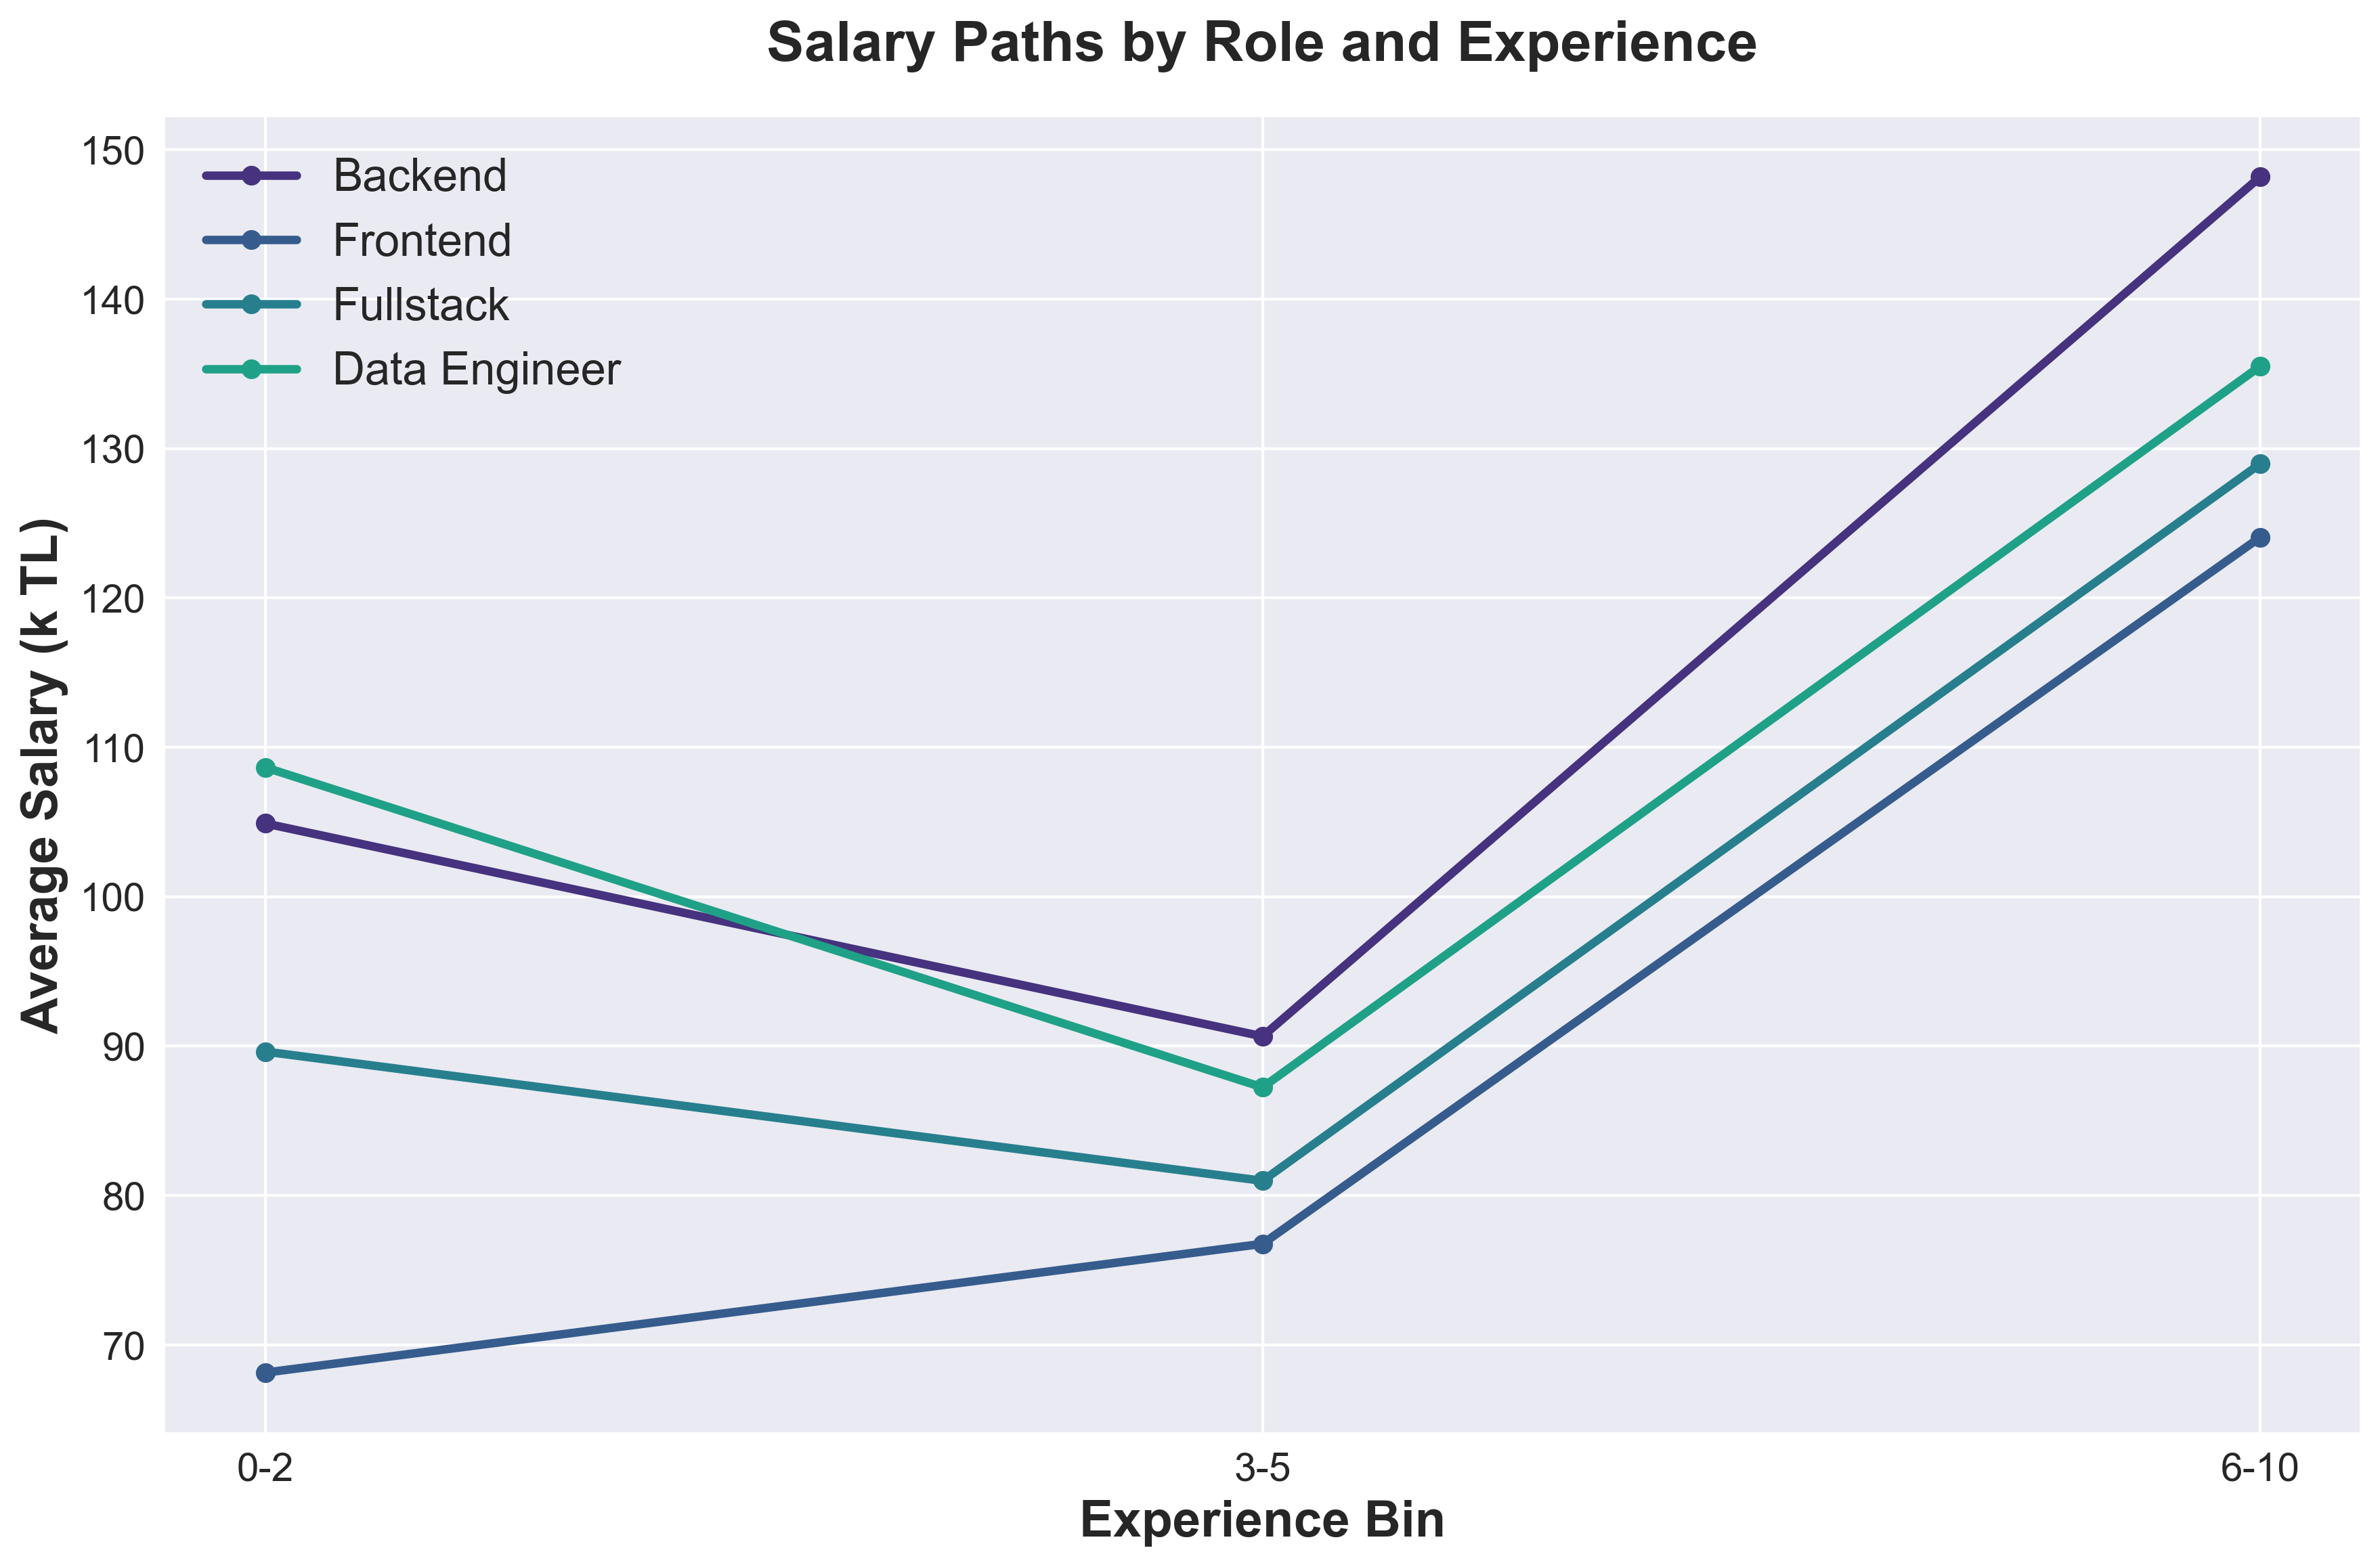
\includegraphics[width=0.85\linewidth]{figures/24_role_experience_salary_paths.png}
  \caption{Salary paths by role and experience.}
  \label{fig:role-exp-salary}
\end{figure}

\begin{figure}[H]
  \centering
  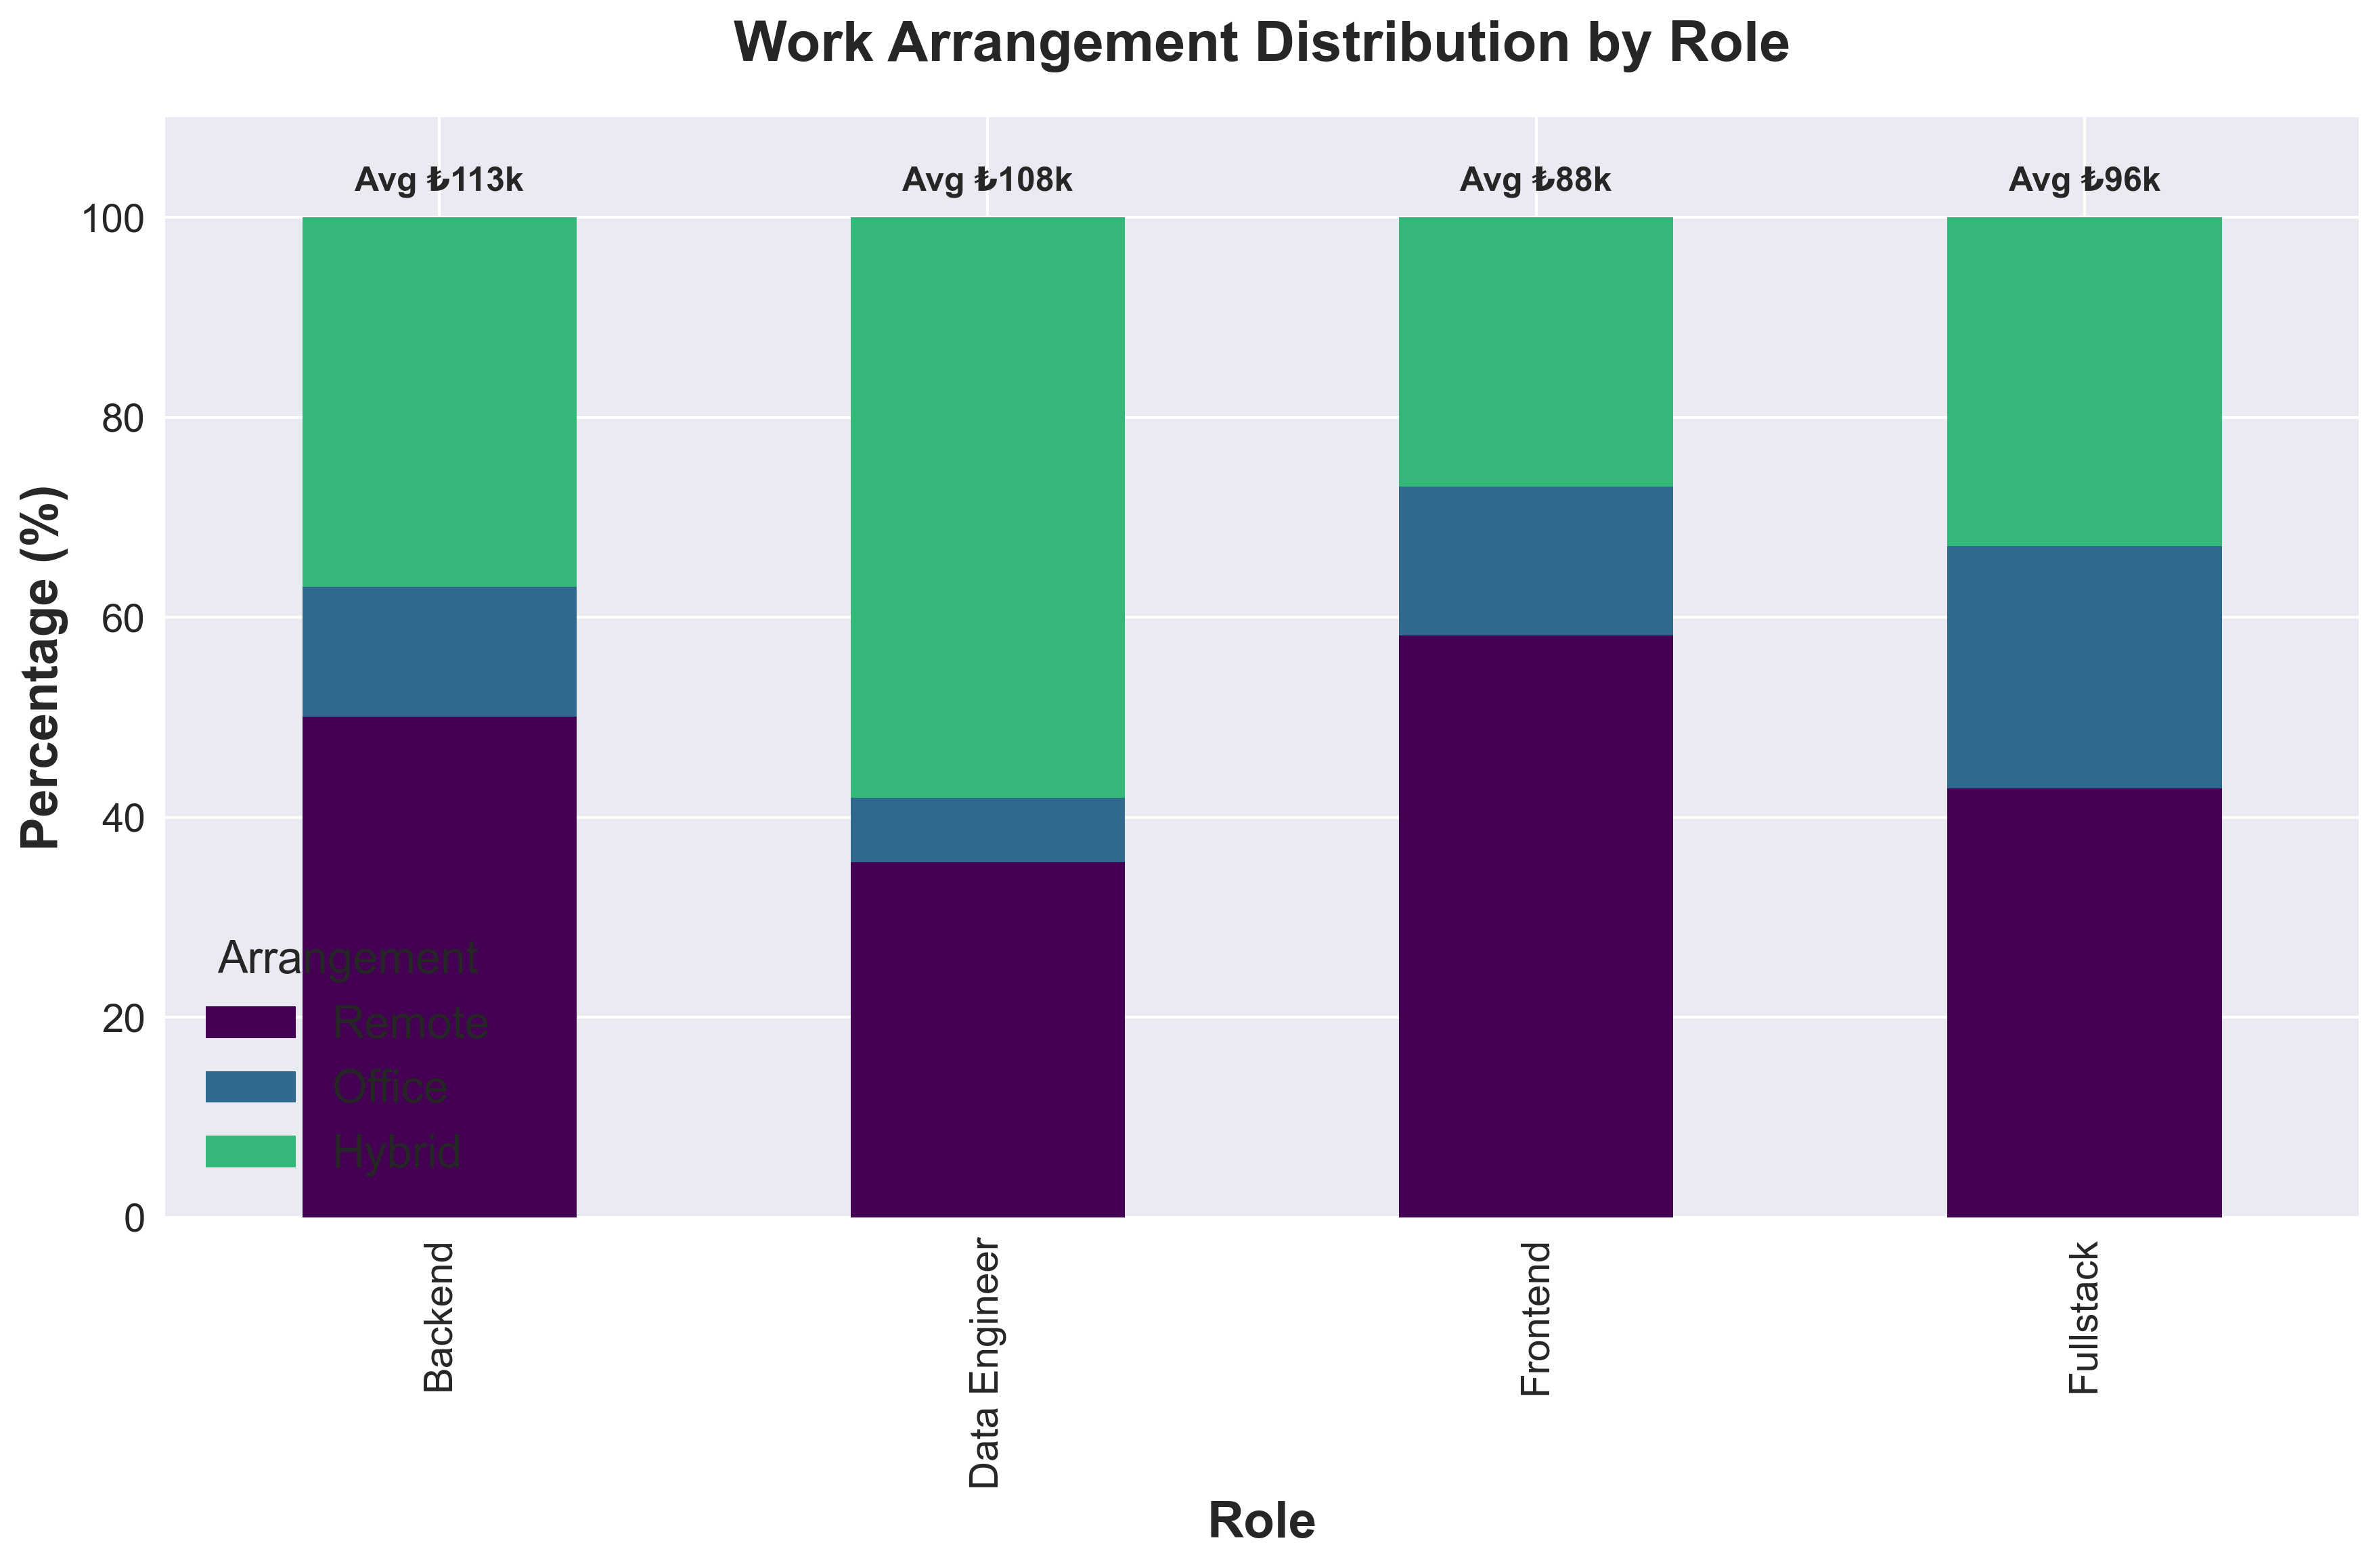
\includegraphics[width=0.85\linewidth]{figures/26_work_arrangement_by_role.png}
  \caption{Work arrangement distribution by role with average salary annotations.}
  \label{fig:work-arrangement-role}
\end{figure}

\begin{figure}[H]
  \centering
  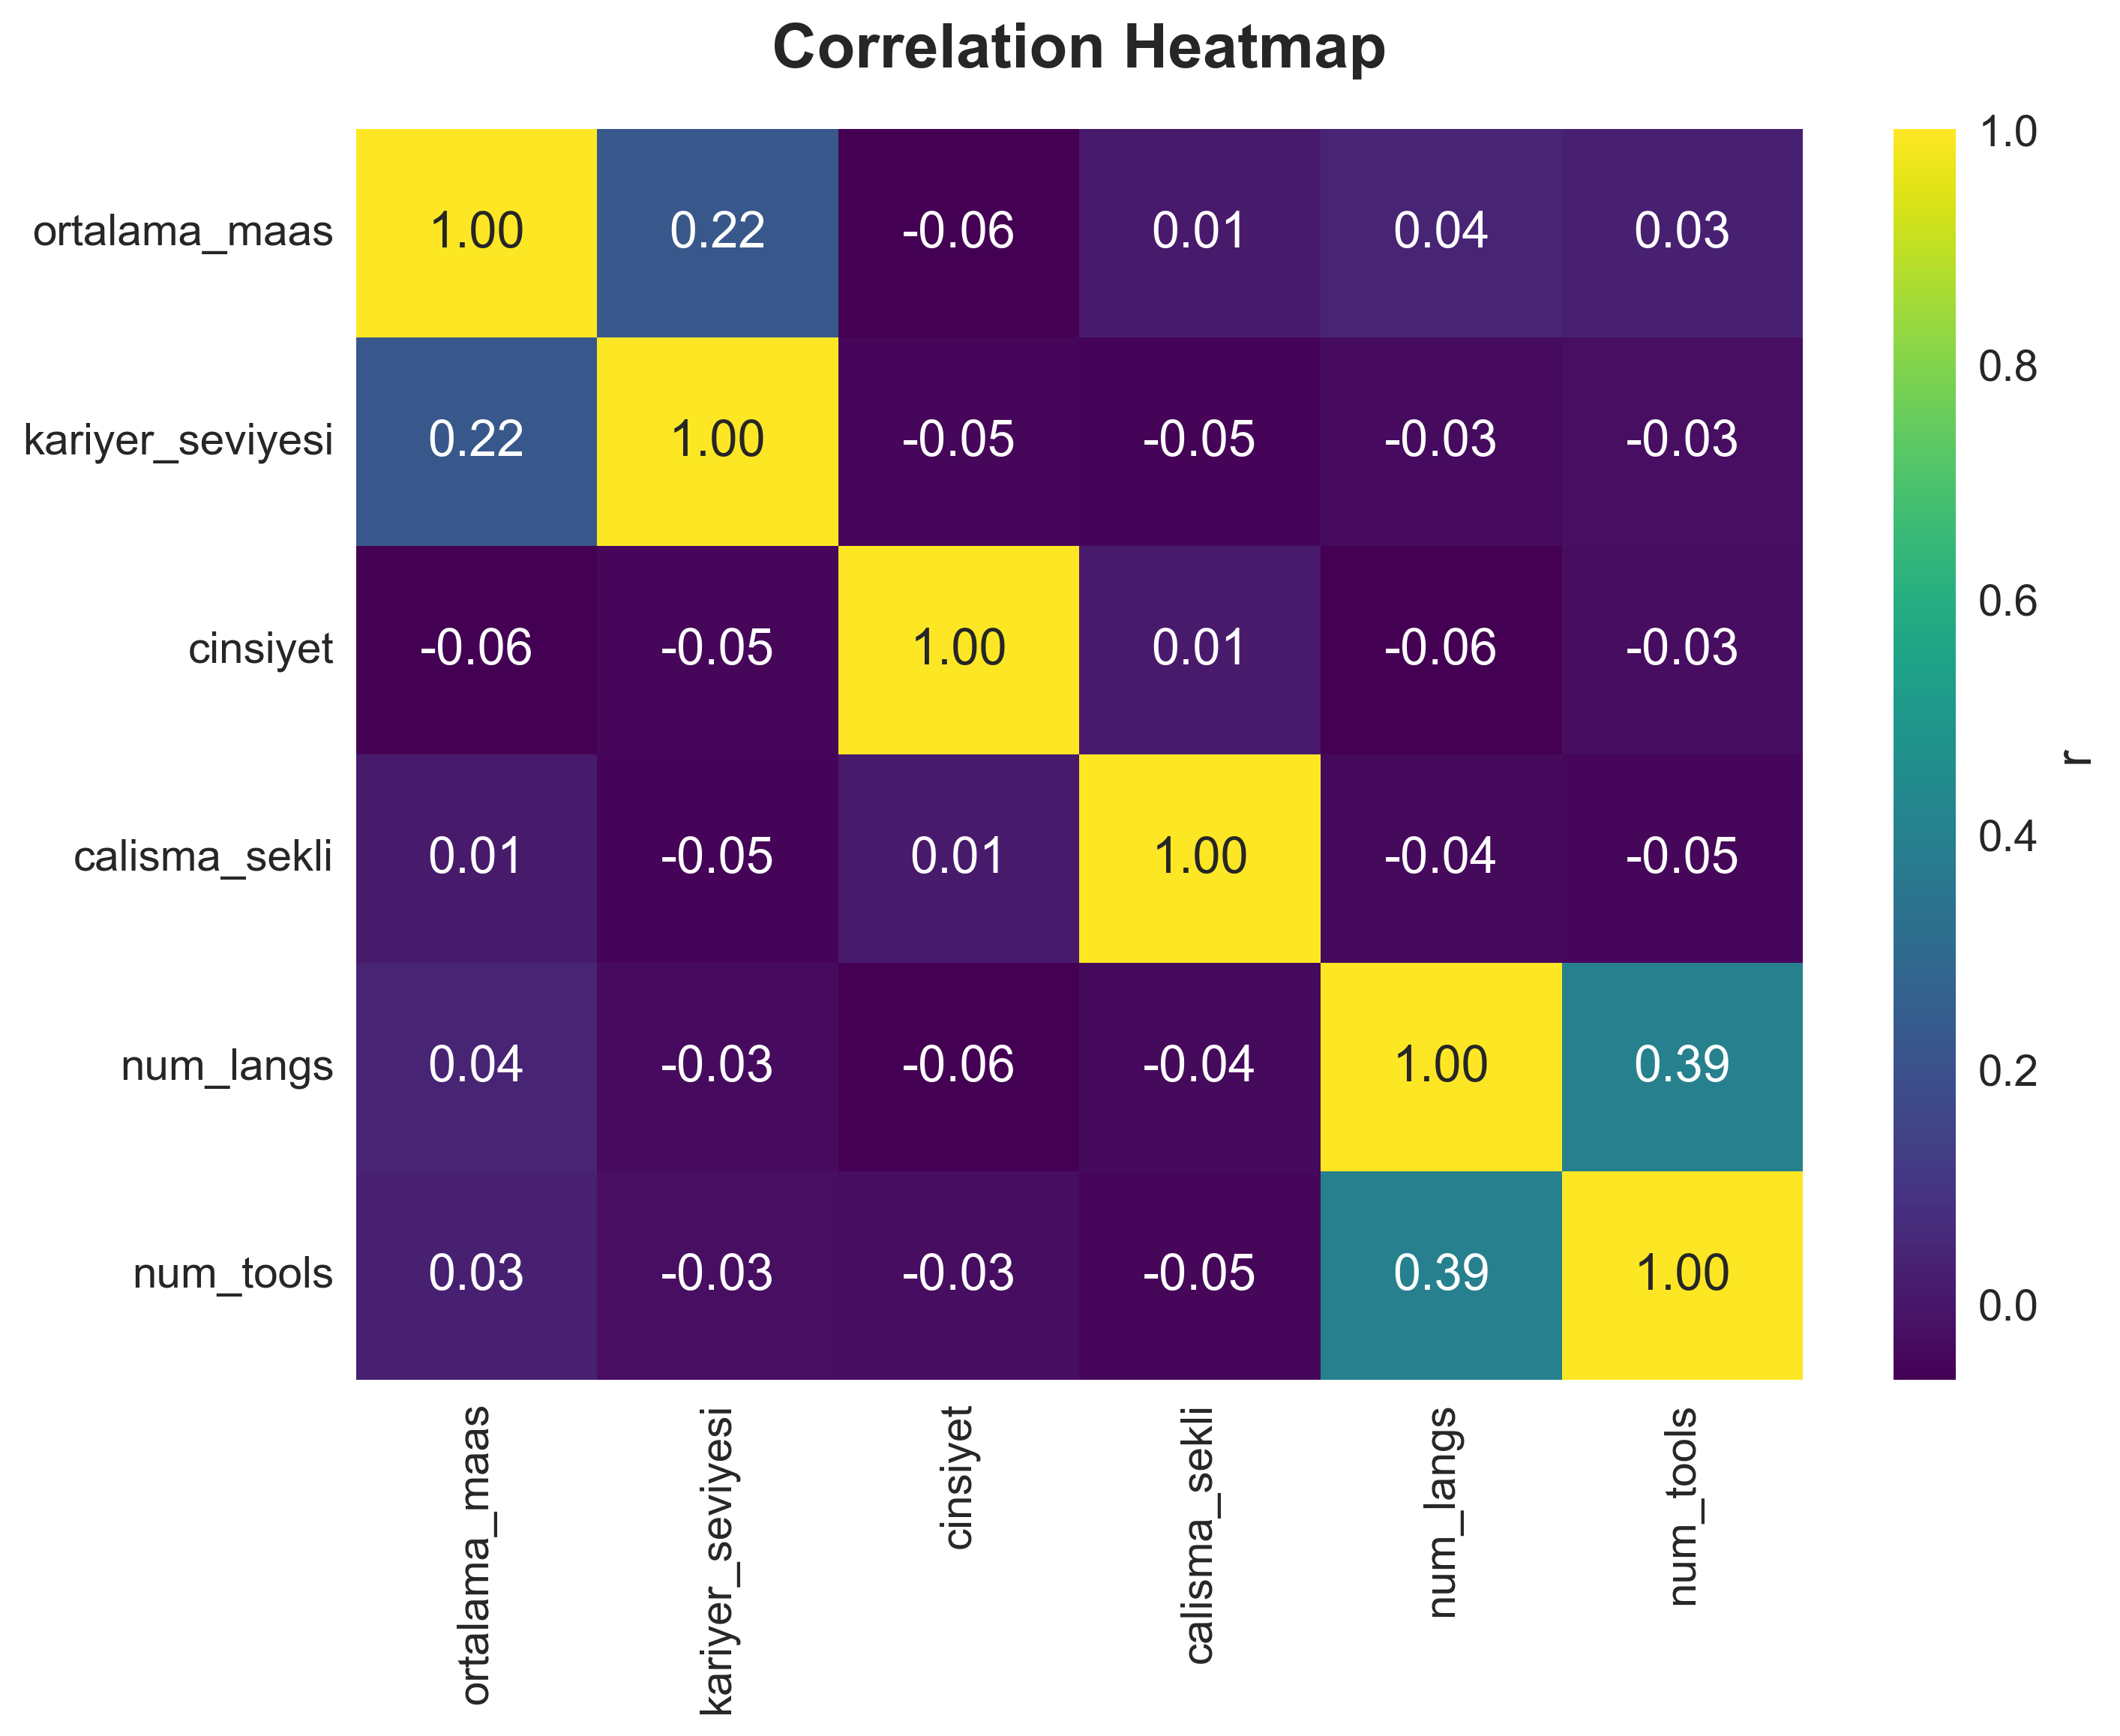
\includegraphics[width=0.85\linewidth]{figures/27_correlation_heatmap.png}
  \caption{Correlation heatmap across selected variables.}
  \label{fig:corr-heatmap}
\end{figure}

\begin{figure}[H]
  \centering
  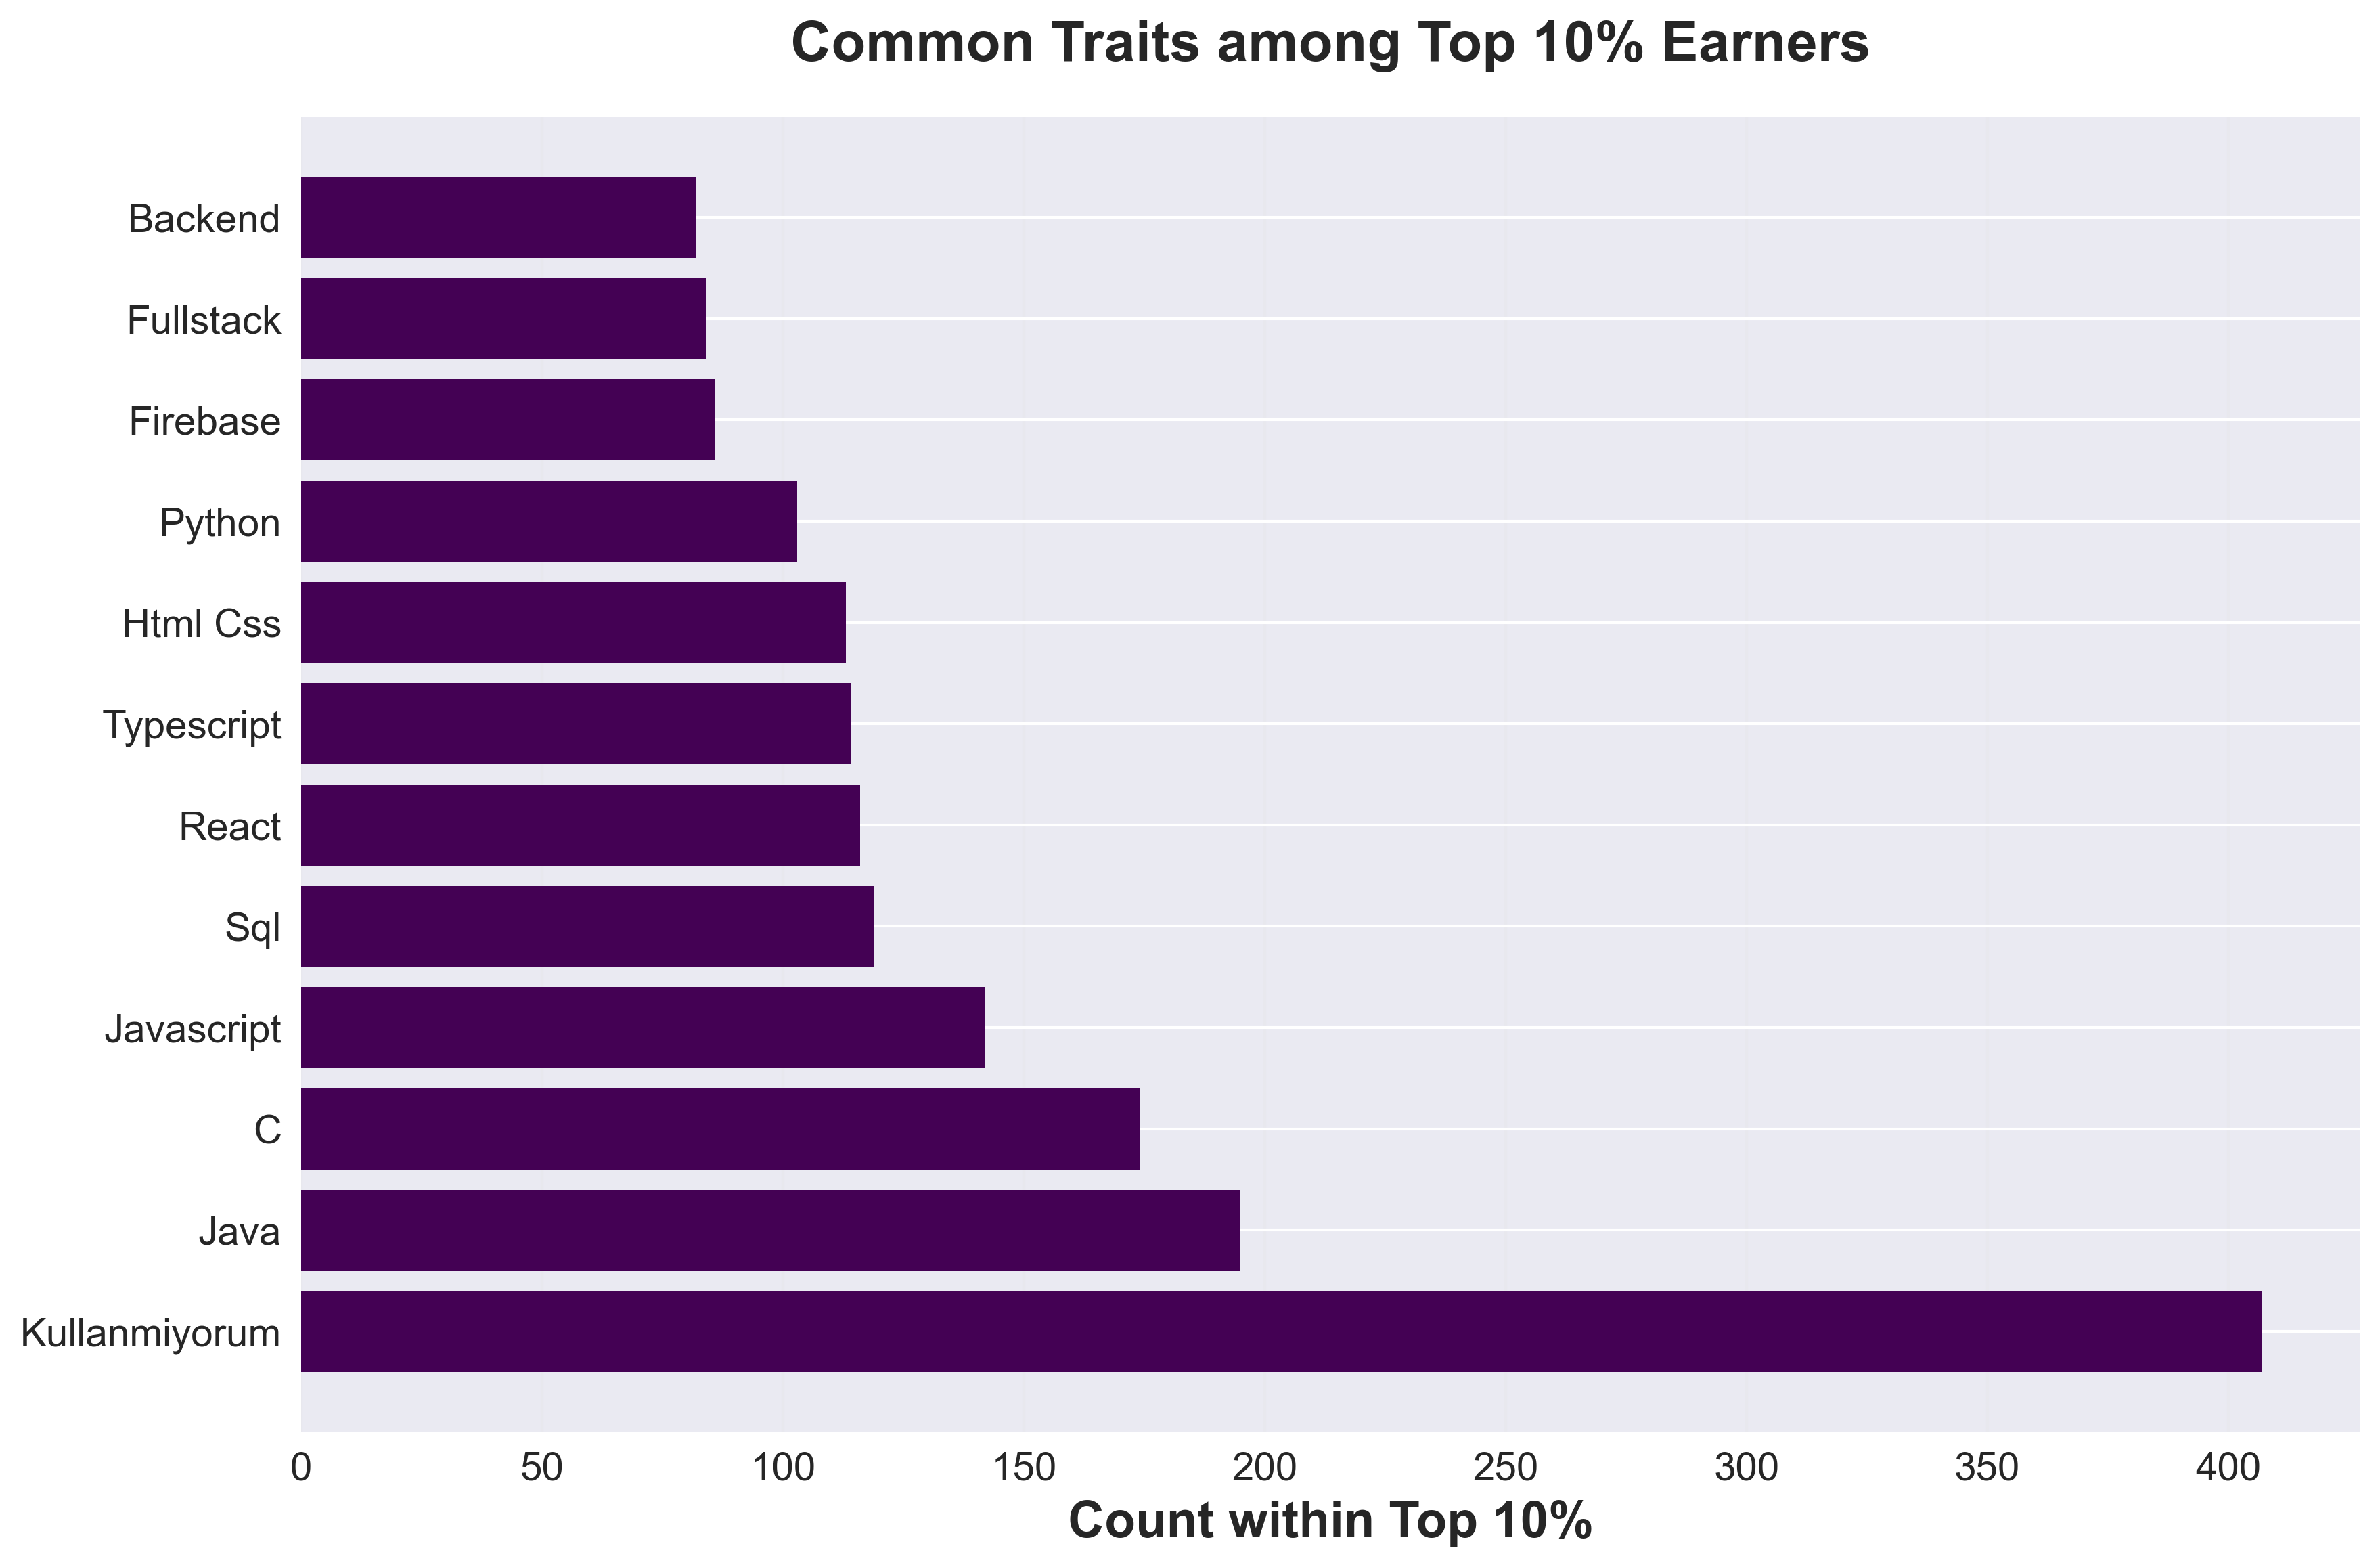
\includegraphics[width=0.85\linewidth]{figures/28_top_earners_traits.png}
  \caption{Common traits among top 10\% earners.}
  \label{fig:top-earners}
\end{figure}


% ================================================================
\section{Discussion}
The findings from this comprehensive salary survey reveal several important patterns and relationships that warrant deeper discussion. This section interprets the results in the context of existing literature, examines unexpected findings, and explores the broader implications for the software sector.

\subsection*{Interpretation of Key Findings}

\textbf{Location as Primary Determinant:} The strong association between company location and salary outcomes aligns with global patterns in the software industry, where international companies typically offer higher compensation than local firms. This finding suggests that the market follows established international norms, with multinational corporations providing premium compensation to attract and retain talent in competitive markets.

\textbf{Gender Pay Gap Significance:} The observed 16\% gender pay gap is consistent with broader technology industry trends but remains concerning. This finding aligns with international studies showing persistent gender disparities in STEM fields, suggesting that despite industry growth, systemic issues in compensation equity persist. The statistical significance of this gap indicates that it is not due to random variation and requires targeted intervention.

\textbf{Technology Stack Synergy:} The finding that technology combinations rather than individual technologies correlate with higher compensation challenges the common narrative of single-technology specialization. This suggests that the market values versatility and the ability to work across different technology domains, reflecting the increasingly complex nature of modern software development.

\subsection*{Comparison with Expectations and Literature}

\textbf{React Usage Findings:} The lack of significant salary difference between React users and non-users contradicts common industry perceptions about the premium value of popular frameworks. This finding suggests that while React remains widely used, its market saturation may have reduced its differentiating value in compensation negotiations.

\textbf{Work Arrangement Effects:} The positive association between remote/hybrid work and salary aligns with recent global trends but may reflect selection effects where higher-paid professionals have more flexibility in work arrangements. This finding supports the growing acceptance of remote work as a viable and potentially beneficial arrangement.

\textbf{Career Progression Patterns:} The clear salary progression across career levels matches established career development models and suggests that the market follows predictable advancement patterns, providing professionals with clear pathways for growth.

\subsection*{Unexpected Findings and Implications}

\textbf{Technology Stack Complexity:} The finding that diversified technology skills correlate with higher compensation suggests that the market increasingly values generalist capabilities over deep specialization in single technologies. This has important implications for educational curricula and professional development strategies.

\textbf{Location Premium Magnitude:} The substantial impact of company location on salary outcomes suggests that geographic factors play a more significant role than previously understood in this context. This finding has implications for talent distribution and regional development policies.

\subsection*{Theoretical and Practical Implications}

\textbf{For Human Capital Theory:} The findings support the view that compensation reflects not just individual skills but also market positioning, company characteristics, and broader economic factors. The strong location effect suggests that institutional and market factors significantly influence individual compensation outcomes.

\textbf{For Compensation Strategy:} Companies should consider location-adjusted compensation policies and focus on creating competitive advantages beyond salary, such as work flexibility and technology diversity opportunities.

\textbf{For Professional Development:} The technology stack findings suggest that professionals should prioritize building diverse skill sets rather than deep specialization in single technologies, particularly in the early stages of their careers.

\subsection*{Limitations and Future Research Directions}

While this study provides valuable insights, several limitations should be acknowledged. The cross-sectional nature of the data limits causal inference, and self-reported salary data may introduce measurement error. Future research should consider longitudinal designs and objective compensation data to strengthen causal claims.

The findings also suggest several promising areas for future investigation, including the role of company size and funding status in compensation patterns, the impact of educational background on salary outcomes, and the evolution of technology stack preferences over time.


% ================================================================
\section{Limitations}
Results reflect the sample composition and self-reported data. While rigorous cleaning and standardization were applied, unobserved confounding and response biases may remain. The ROI analysis is correlational and should not be interpreted causally.


% ================================================================
\section{Conclusion and Recommendations}
Company location and work arrangement are strongly associated with salary outcomes, with the largest differences across locations and a medium effect by work arrangement. A statistically significant gender pay gap of approximately 16\% is observed. React usage alone does not imply higher pay; rather, broader stack combinations correlate with stronger outcomes. These insights inform compensation policy, career decisions, and talent strategy.

\subsection{Future Work}
Building upon the findings of this salary survey, we outline two focused directions for future work that align with the project documentation and practical next steps:

\subsection*{Comparison with Global Benchmarks}

\textbf{Stack Overflow Dataset Alignment:} Compare key metrics (salary distribution, technology usage, work arrangement effects, gender gap) with recent global Stack Overflow Developer Survey data. This will contextualize findings, quantify similarities/differences, and identify where local patterns diverge from global benchmarks.

\subsection*{Salary Prediction Model}

\textbf{Predictive Modeling:} Develop a transparent, reproducible salary prediction model using the cleaned dataset. Begin with interpretable baselines (regularized linear models, GAMs), then evaluate tree-based approaches (Random Forest, XGBoost) with careful cross-validation. Report performance (MAE/RMSE), feature importance, calibration, and fairness diagnostics (e.g., group-wise error).

These two directions provide high-impact, tractable extensions that directly build on the current analysis without introducing unnecessary scope or complexity.


% ================================================================
\section*{Acknowledgments}
We thank all survey participants and contributors to data processing, analysis, visualization, and the Streamlit dashboard.


% ================================================================
\appendix
\section{Visualization Standards}
All figures comply with the shared styling guide: consistent fonts, color palette, axis labeling, and 300 DPI resolution. Files are named in snake\_case and stored in \texttt{reports/latex\_report/figures}. The dashboard reuses the same conventions for visual coherence across media.


\section{Reproducibility and Technical Stack}
Analyses were implemented in Python using pandas, NumPy, SciPy, statsmodels, seaborn, and matplotlib. Reproducibility is supported via versioned source files in \texttt{src/}, notebooks in \texttt{notebooks/}, and pinned dependencies in \texttt{requirements.txt}. Interactive exploration is provided by a Streamlit app (\texttt{app.py}).


\section{Project Management}
Work proceeded in five sprints, each with well-defined deliverables: data preparation; core hypothesis testing; secondary analyses and visualization drafts; publication-quality visualization and dashboard; and final reporting. All sprint objectives and outputs are documented in the project plan and associated markdown files under \texttt{docs/}.


% ================================================================
\begin{thebibliography}{9}
\bibitem{wilcox2012} R. R. Wilcox. \textit{Introduction to Robust Estimation and Hypothesis Testing}. Academic Press, 2012.
\bibitem{cohen1988} J. Cohen. \textit{Statistical Power Analysis for the Behavioral Sciences}. Lawrence Erlbaum, 1988.
\bibitem{field2013} A. Field. \textit{Discovering Statistics Using IBM SPSS Statistics}. Sage, 2013.
\bibitem{wasserman2004} L. Wasserman. \textit{All of Statistics}. Springer, 2004.
\bibitem{tukeyHSD} H. Abdi and L. J. Williams. “Tukey’s Honestly Significant Difference (HSD) Test.” In: \textit{Encyclopedia of Research Design}, 2010.
\bibitem{seaborn} M. Waskom. “Seaborn: Statistical Data Visualization.” \textit{Journal of Open Source Software}, 2021.
\bibitem{pandas} W. McKinney. “Data Structures for Statistical Computing in Python.” \textit{Proceedings of the 9th Python in Science Conference}, 2010.
\bibitem{scipy} P. Virtanen et al. “SciPy 1.0: Fundamental Algorithms for Scientific Computing in Python.” \textit{Nature Methods}, 2020.
\end{thebibliography}


\end{document}